\documentclass[11pt,a4paper,oneside,hidelinks]{scrartcl}
\setlength{\parindent}{0pt}

\usepackage{fixltx2e}%% the official fixes for LaTeX2e
\usepackage[a4paper,left=1in, right=1in, top=1in, bottom=1in]{geometry}
%\usepackage[draft]{graphicx} %% add [draft] for not generating figures (compiles much faster, in case only want to see text)
\usepackage{graphicx}
\usepackage{color}
\usepackage{float}
\usepackage{amsmath}
\usepackage{amssymb}
\usepackage{soul} %% use \hl to higlight text
\usepackage[section]{placeins} %% use \FloatBarrier command  to prevent floats to appear beyond some point in your documen
\usepackage{enumitem}
\usepackage[xetex]{attachfile2} %% note to not put underscores in filenames and use only with pdf->latex
\usepackage{textcomp}
\attachfilesetup{color=0 0 1,print=true}

\newcommand\Rey{\mbox{\textit{Re}}\,\,}
\newcommand\bfr[1]{\textcolor[rgb]{1,0.00,0.00}{\textbf{\textsf{#1}}}}
\newcommand\ra{$\rightarrow$}
\newcommand\cm{\textcolor[rgb]{0.00,0.50,0.00}{\checkmark}\,\,}
\begin{document}

EG501V Computational Fluid Dynamics (2017/2018)
\\
\\
\textbf{Practical 1b: CFD modeling of laminar flow using ANSYS Fluent}

\section{Introduction}
This practical shows how to solve the basic problem of fluid flow through a circular pipe. Two laminar flow scenarios are considered: (1) laminar flow in a pipe and (2) start-up flow between to parallel plates. The {\bf learning outcomes} of this tutorial cover four key elements involving CFD simulation and  analysis:
\begin{enumerate}
  \item Build up model's \emph{Geometry};
  \item \emph{Mesh generation};
  \item Performing the \emph{Fluent analysis}, and
  \item \emph{Post-processing} of results.
\end{enumerate}
This tutorial will guide you step-by-step through these four procedures and provide basic skill sets to complete the assignment.

\section{Laminar pipe flow}\label{Section:LaminarPipeSimple}
Consider a fluid flowing through a circular pipe of diameter $D$ and length $L$ as sketched below. The pipe diameter is $D=0.3$\,m and the length of the pipe is $L=6$\,m. The inlet velocity  is constant over the cross-section and is equal to $U=1$\,m/s. The  fluid density is $\rho=1$\,kg/m$^3$ and the fluid viscosity is $\mu=1.5\times10^{-3}$\,kg/ms. Note that these properties result in a Reynolds number of $\Rey=\rho DL/\mu=200$ which means the flow is laminar. The outlet pressure $p_\mathrm{o}$ is equal to 1 atmosphere (standard pressure).\\
\begin{center}
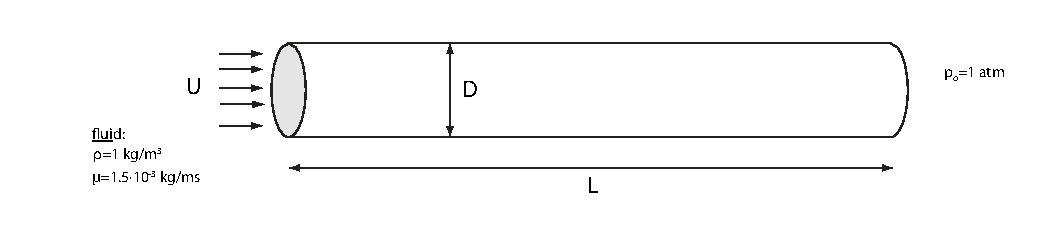
\includegraphics[width=\textwidth,clip]{pipe_sketch.pdf}
\end{center}

Solve this flow problem using ANSYS Fluent and present the following results:
\begin{itemize}
\item velocity vectors
\item velocity magnitude contours
\item velocity profiles
\item skin friction coefficient along the pipe wall
\end{itemize}

Note that the physical problem of flow in a pipe is a 3D problem, however because the flow across any plane passing through the centreline of the pipe is identical we can model the flow in 2Dimendions. Moreover because in this ``slice'' of dimensions $D\times L$ the flow is symmetrical around the centreline we only need to simulate the flow in one half of the plane of dimensions $r\times L$. Flows which are symmetrical around a centreline are also called \emph{axisymmetric} flows and by modelling it in 2D we save considerable computational resources compared to full 3D simulations.


\subsection{Starting ANSYS workbench}

Prior to opening ANSYS, create a folder (e.g. FluentCFD) on your \emph{Homedrive}. This folder will be used to store the files created during this session, and allow you to reopen them at a later stage. You will need approximately 10\,MB of free space for this tutorial, so make sure this space is available on your \emph{Homedrive}.\\

On the desktop go to the folder \bfr{Physical Sciences\ra Engineering\ra ANSYS 18.1} and double click the shortcut \bfr{Workbench 18.1}, see the figure below \hl{need to replace with 18.1}.

%\begin{figure}[H]
%\begin{center}
%\includegraphics[width=.8\textwidth,clip]{desktop.png}
%\end{center}
%\end{figure}

You should now see a window as in the figure below.

\begin{figure}[H]
\begin{center}
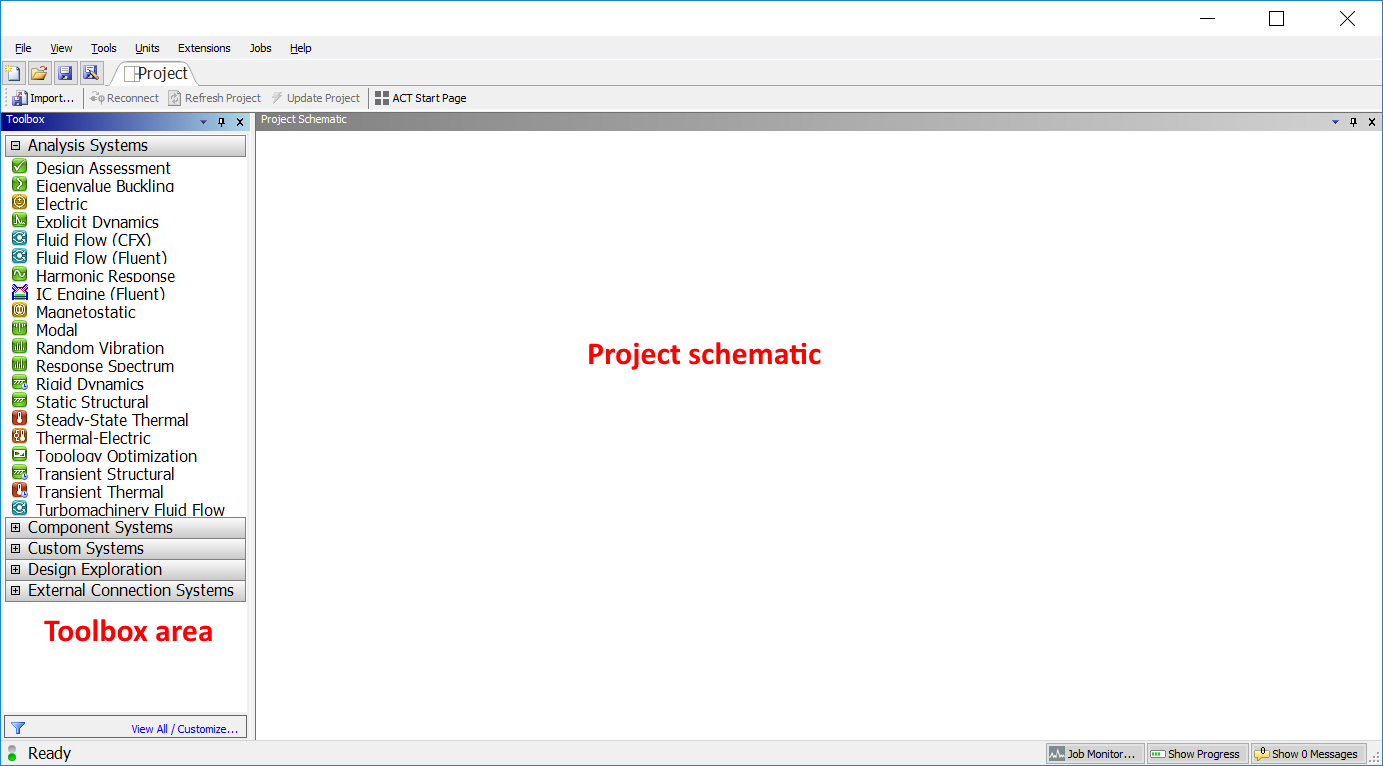
\includegraphics[width=.7\textwidth,clip]{workbench.png}
\end{center}
\end{figure}

This is the ANSYS workbench which consists primarily of the \emph{Toolbox area} (left column) and the \emph{Project schematic} in the main area. Above these areas you can find the usual toolbar and the menu bar. The main way to work in the workbench is to drag an item from you toolbox to a desired location in the Project schematic. Alternatively you can double-click any item in the \emph{Toolbox area} and it will appear in the \emph{Project schematic}, although you do not have any control over its location this way (it will appear on the next line). The \emph{Analysis Systems} contain all the necessary components to model a specific problem. So in the case of \emph{Fluid Flow (Fluent)} it contains the following components to complete the fluid flow simulation: \emph{Geometry, Mesh, Setup, Simulation, Results}. The components are automatically linked and you would normally work through these components from top to bottom (i.e. you cannot work on the \emph{Mesh} before the \emph{Geometry} is completed etc.). An example of this is object \emph{A} in the project schematic in the figure below.
Here we are going to set-up our simulation from the individual components in the \emph{Component Systems} menu and establish the links between components ourselves. This gives us greater flexibility at later stages to link for example the same geometry to different meshes (e.g in the figure below geometry or to link the same mesh to different set-ups. An example is shown in bottom part of the project schematic below where geometry component \emph{B} is linked to mesh components \emph{C} and \emph{F}, and mesh component \emph{F} in turn is linked to Fluent set-ups omponent \emph{G} and \emph{I} (do not create this now!).

\begin{figure}[H]
\begin{center}
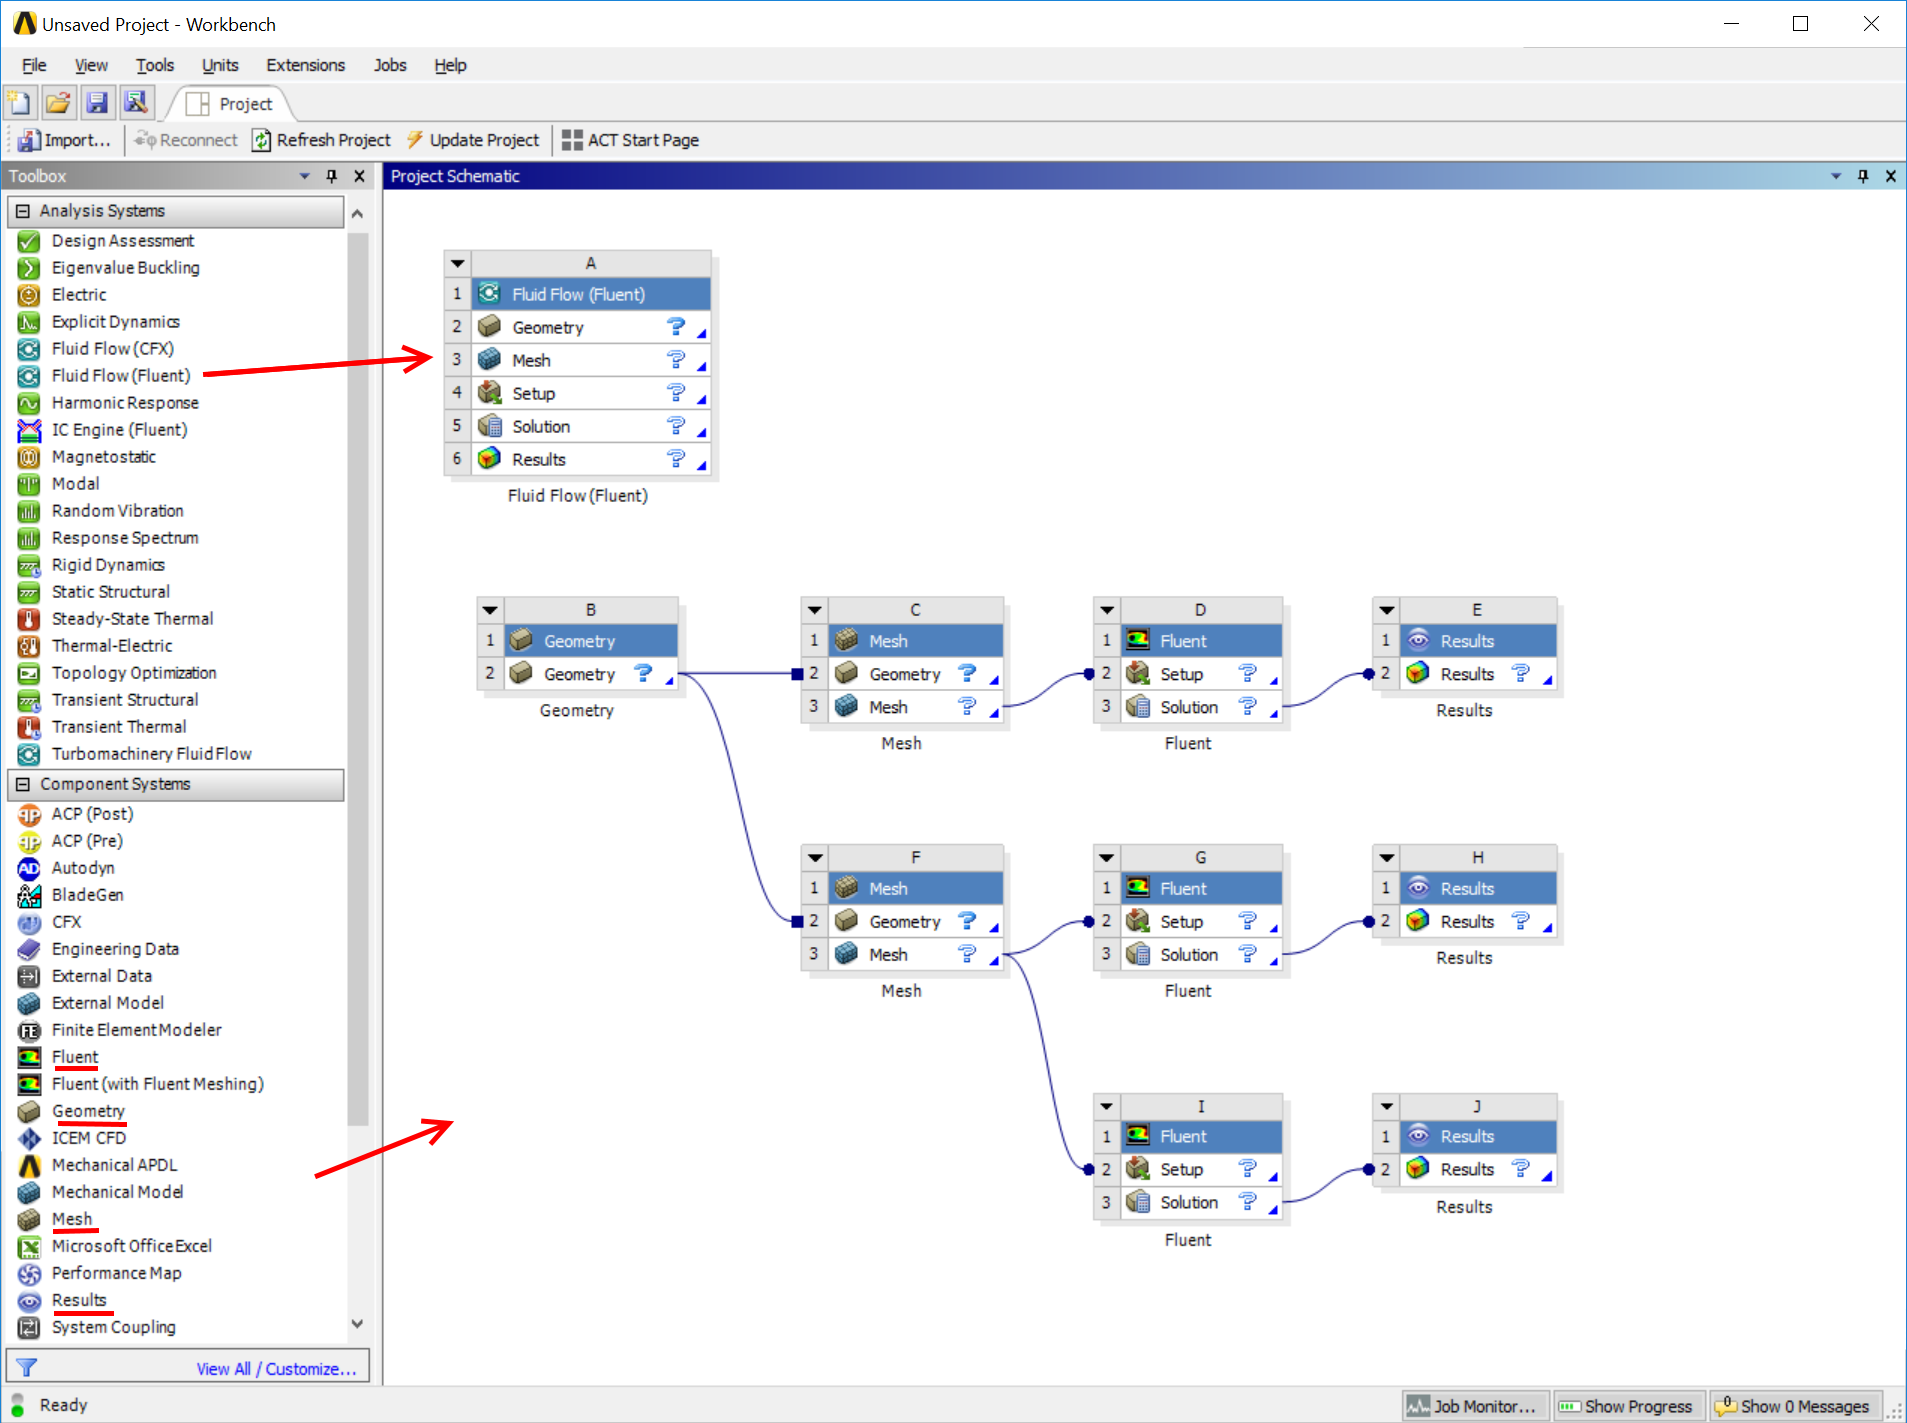
\includegraphics[width=0.65\textwidth,clip]{workbench_components.png}
\end{center}
\end{figure}

\subsection{Geometry}


\subsubsection{Make a sketch}
Now click the boxed $+$ symbol in the \bfr{Component Systems} menu and drag the \bfr{Geometry} component to the Project schematic. Right click the \bfr{Geometry} cell and select \bfr{Properties}. Change the value of \bfr{Analysis type} from the default value 3D into 2D as indicated below.

\begin{figure}[H]
\begin{center}
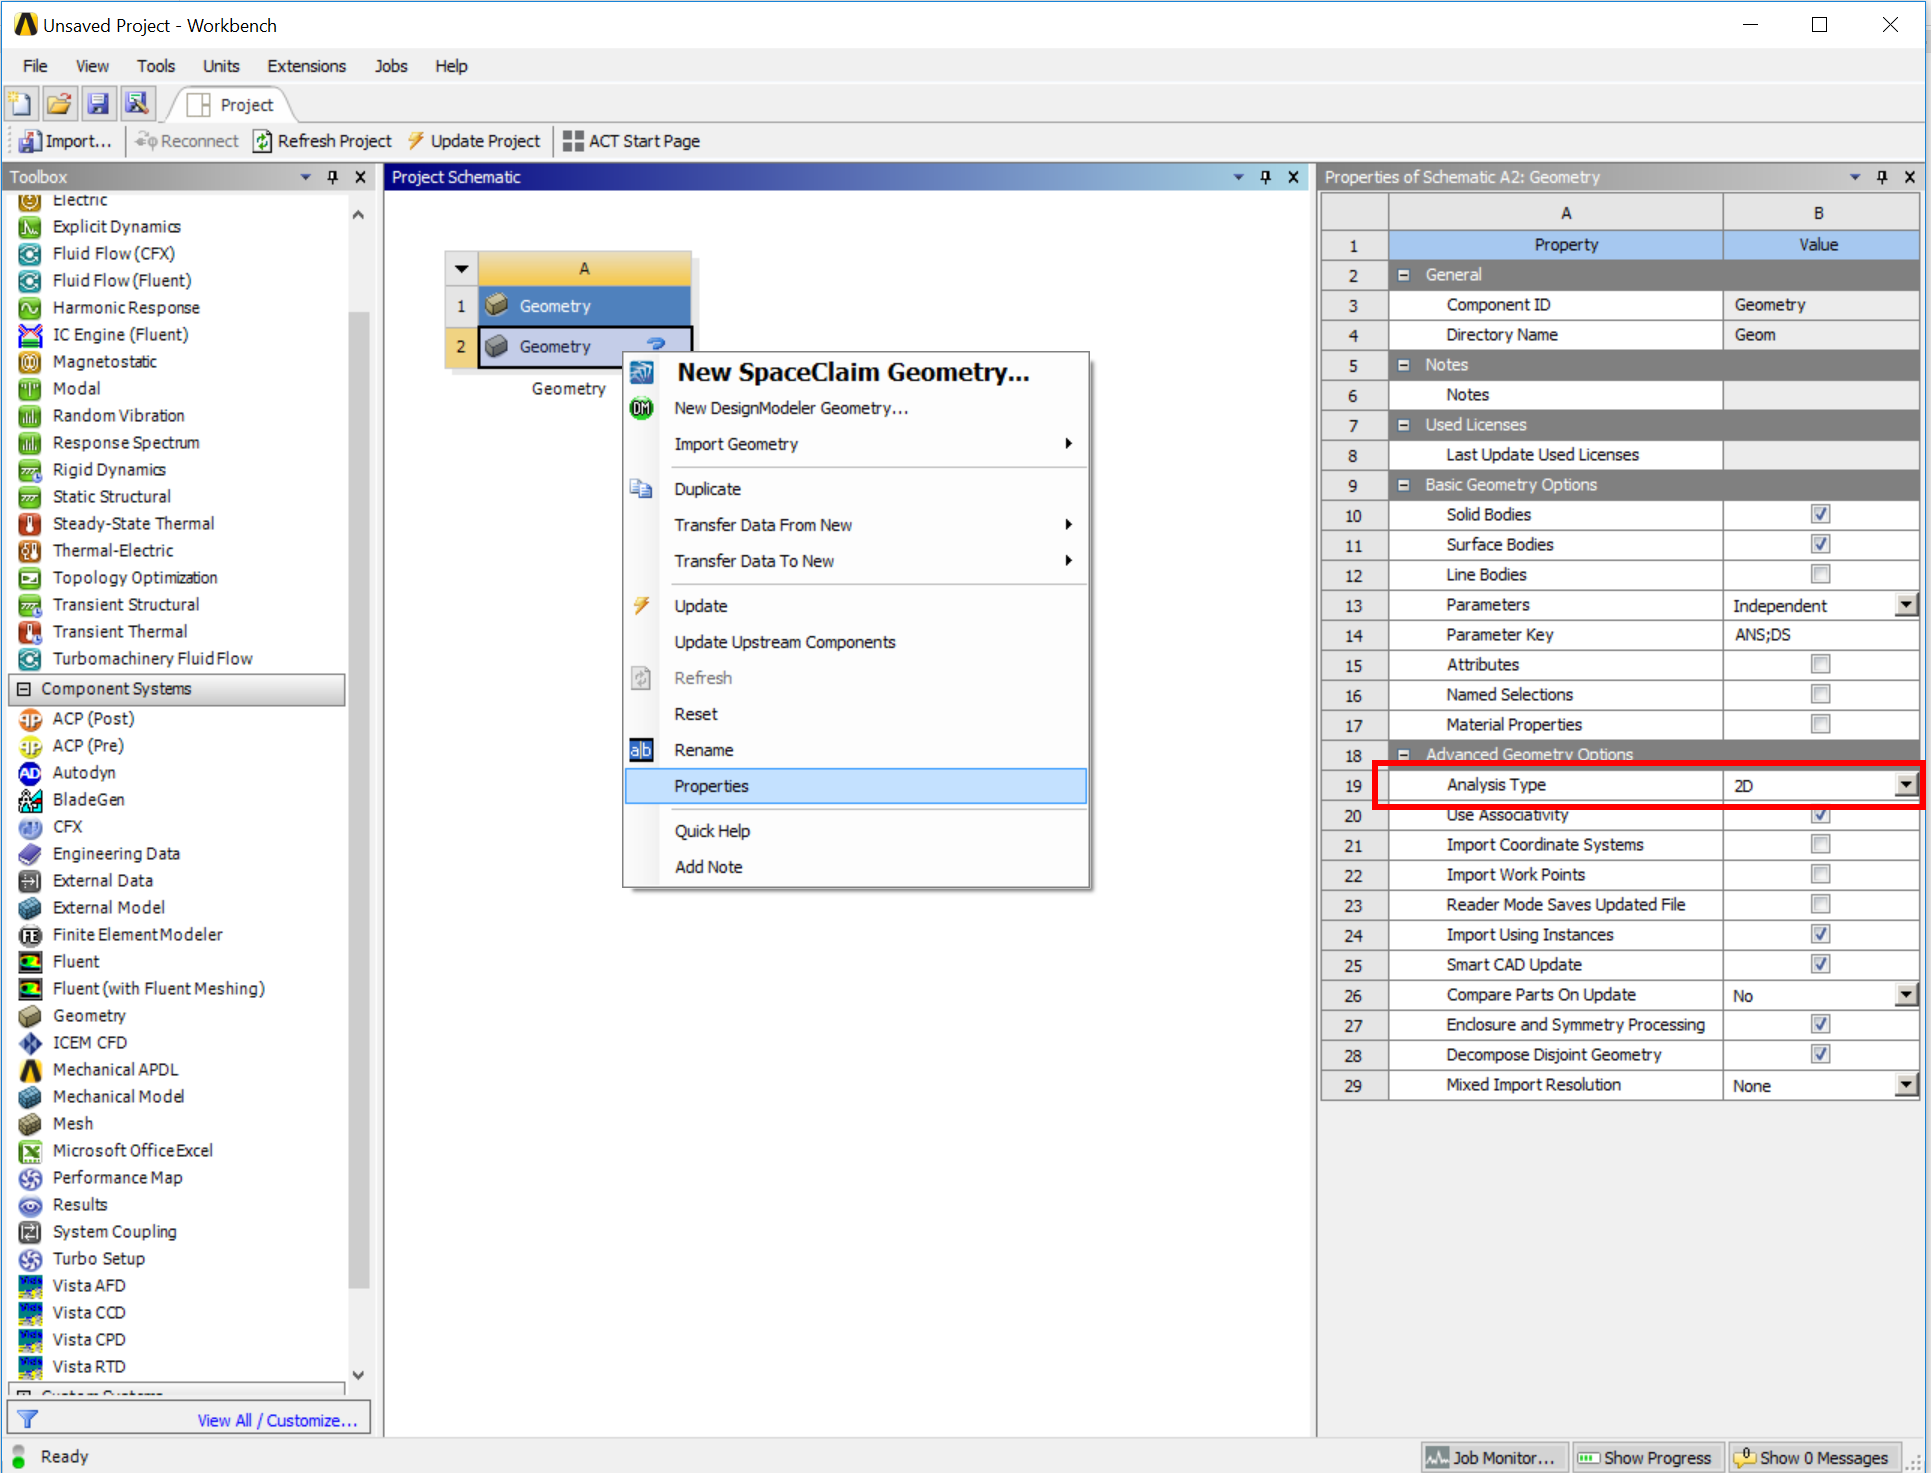
\includegraphics[width=0.7\textwidth,clip]{geometry_analysis_type.png}
\end{center}
\end{figure}

Right-click \bfr{Geometry} again and select the second option \bfr{New DesignModeler Geometry}. We do not choose the default \emph{SpaceClaim} option to make our geometry, \emph{SpaceClaim} is ANSYS's inbuild CAD software (similar to SolidWorks) which can be used to make very complex geometries, but similar to SolidWorks also requires more time to learn. Because in this course we only use very simple geometries, and because learning another CAD package is not the aim of this course, we are going to use the more basic \emph{DesignModeler}.

The \emph{DesignModeler} window will now have appeared. The main areas and toolbars that you will be using are displayed in the image below. We will use these expressions (i.e \emph{Tree outline}, \emph{Details View} etc.), to guide you trough the rest of the geometry section.

\begin{figure}[H]
\begin{center}
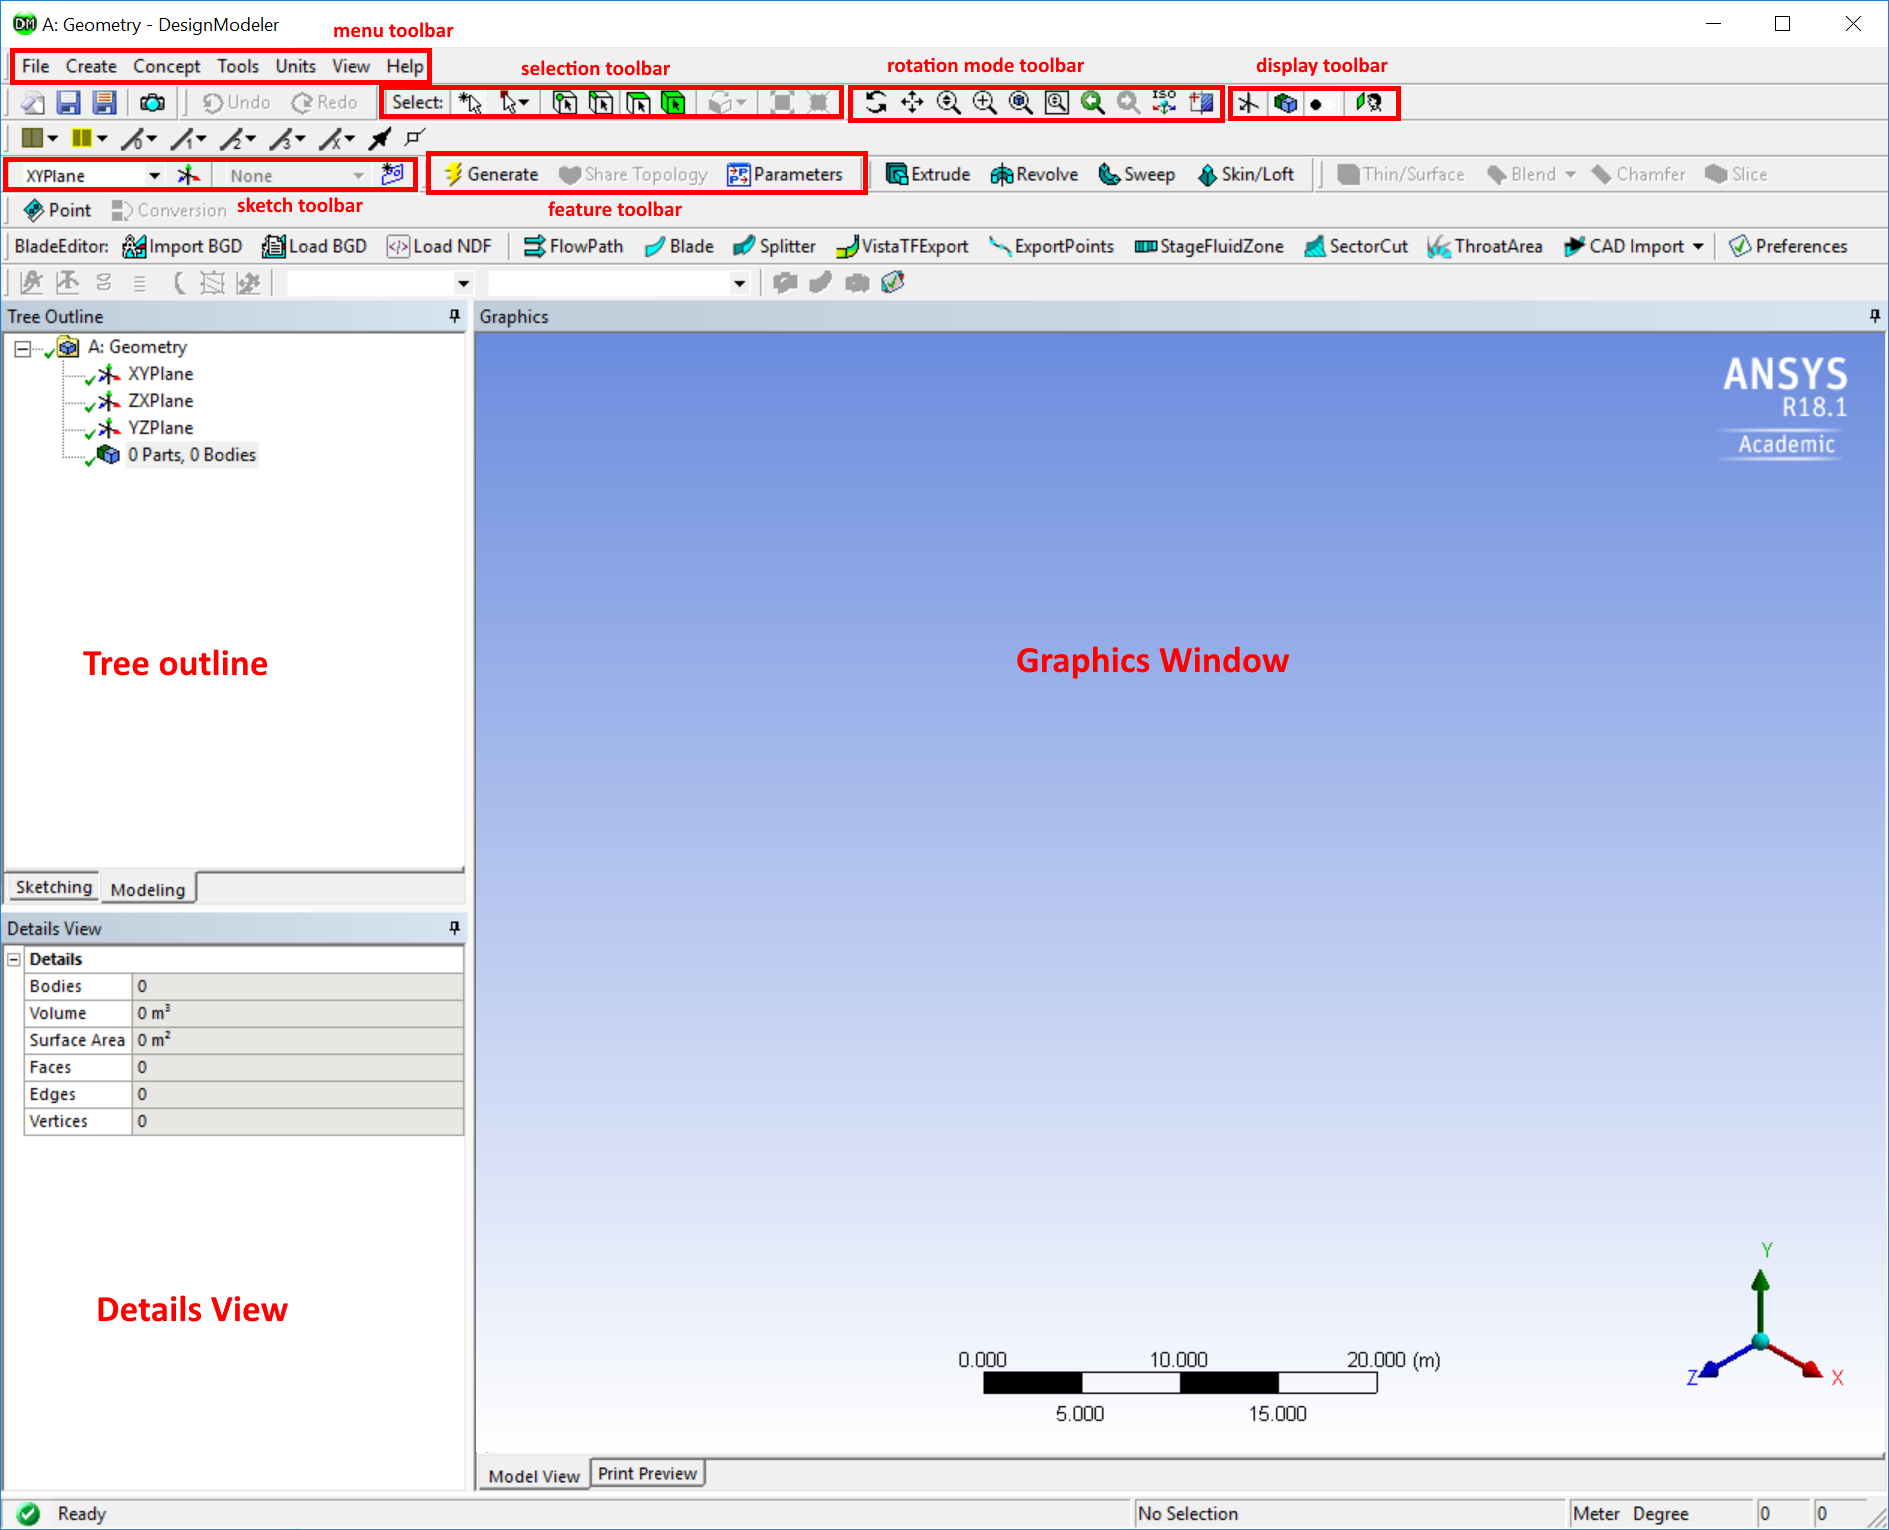
\includegraphics[width=0.7\textwidth,clip]{Designmodeller_GUI.png}
\end{center}
\end{figure}

You will now create a sketch in the XY-plane. First select the \bfr{XYplane} in the \emph{Tree Outline} on the left hand side of your window and click the \bfr{New Sketch} symbol 
\includegraphics[width=.4cm]{newsketch_symbol.png} in the sketch toolbar. \bfr{Sketch1} should now appear under the \bfr{XYPlane} in your \emph{Tree Outline} as shown below.
\begin{figure}[H]
\begin{center}
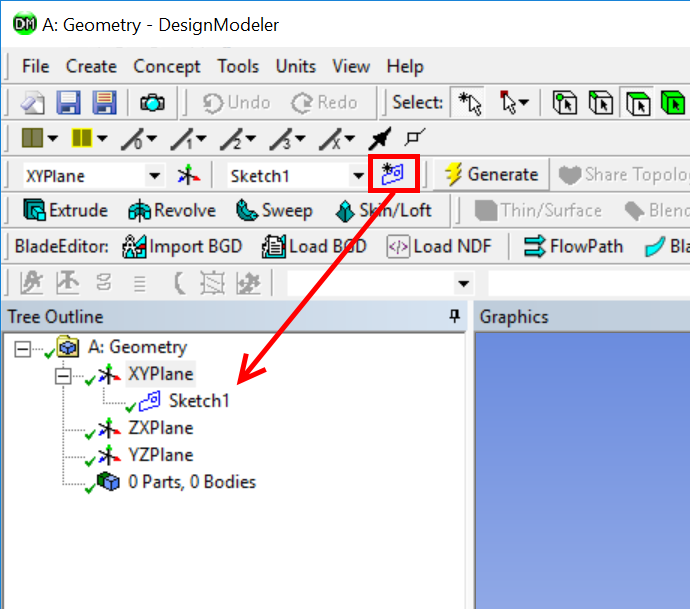
\includegraphics[width=0.4\textwidth,clip]{newsketch.png}
\end{center}
\end{figure}

Next, in the \emph{Graphics Window} click on the \bfr{Z-axis} in the coordinate system to obtain a 2-dimensional view of the \bfr{XYPlane}. Now go to the \bfr{Sketching tab} in the \emph{Tree Outline}, select \bfr{Rectangle} and draw a rectangle in the \emph{Graphics Window} by clicking first on the origin (a ``P'' will appear if you hover the mouse over the origin, this P indicates your mouse pointer is at a point of intersection, similarly a ``C'' will appear of your pointer is on a line - note that the P might be difficult to distinguish in this case since it is overlapped by both axes, the origin and your mouse pointer!). The dimensions of the rectangle (or pipe in this case) do not matter at this stage since we will specify the dimension in the next step.

\begin{figure}[H]
\begin{center}
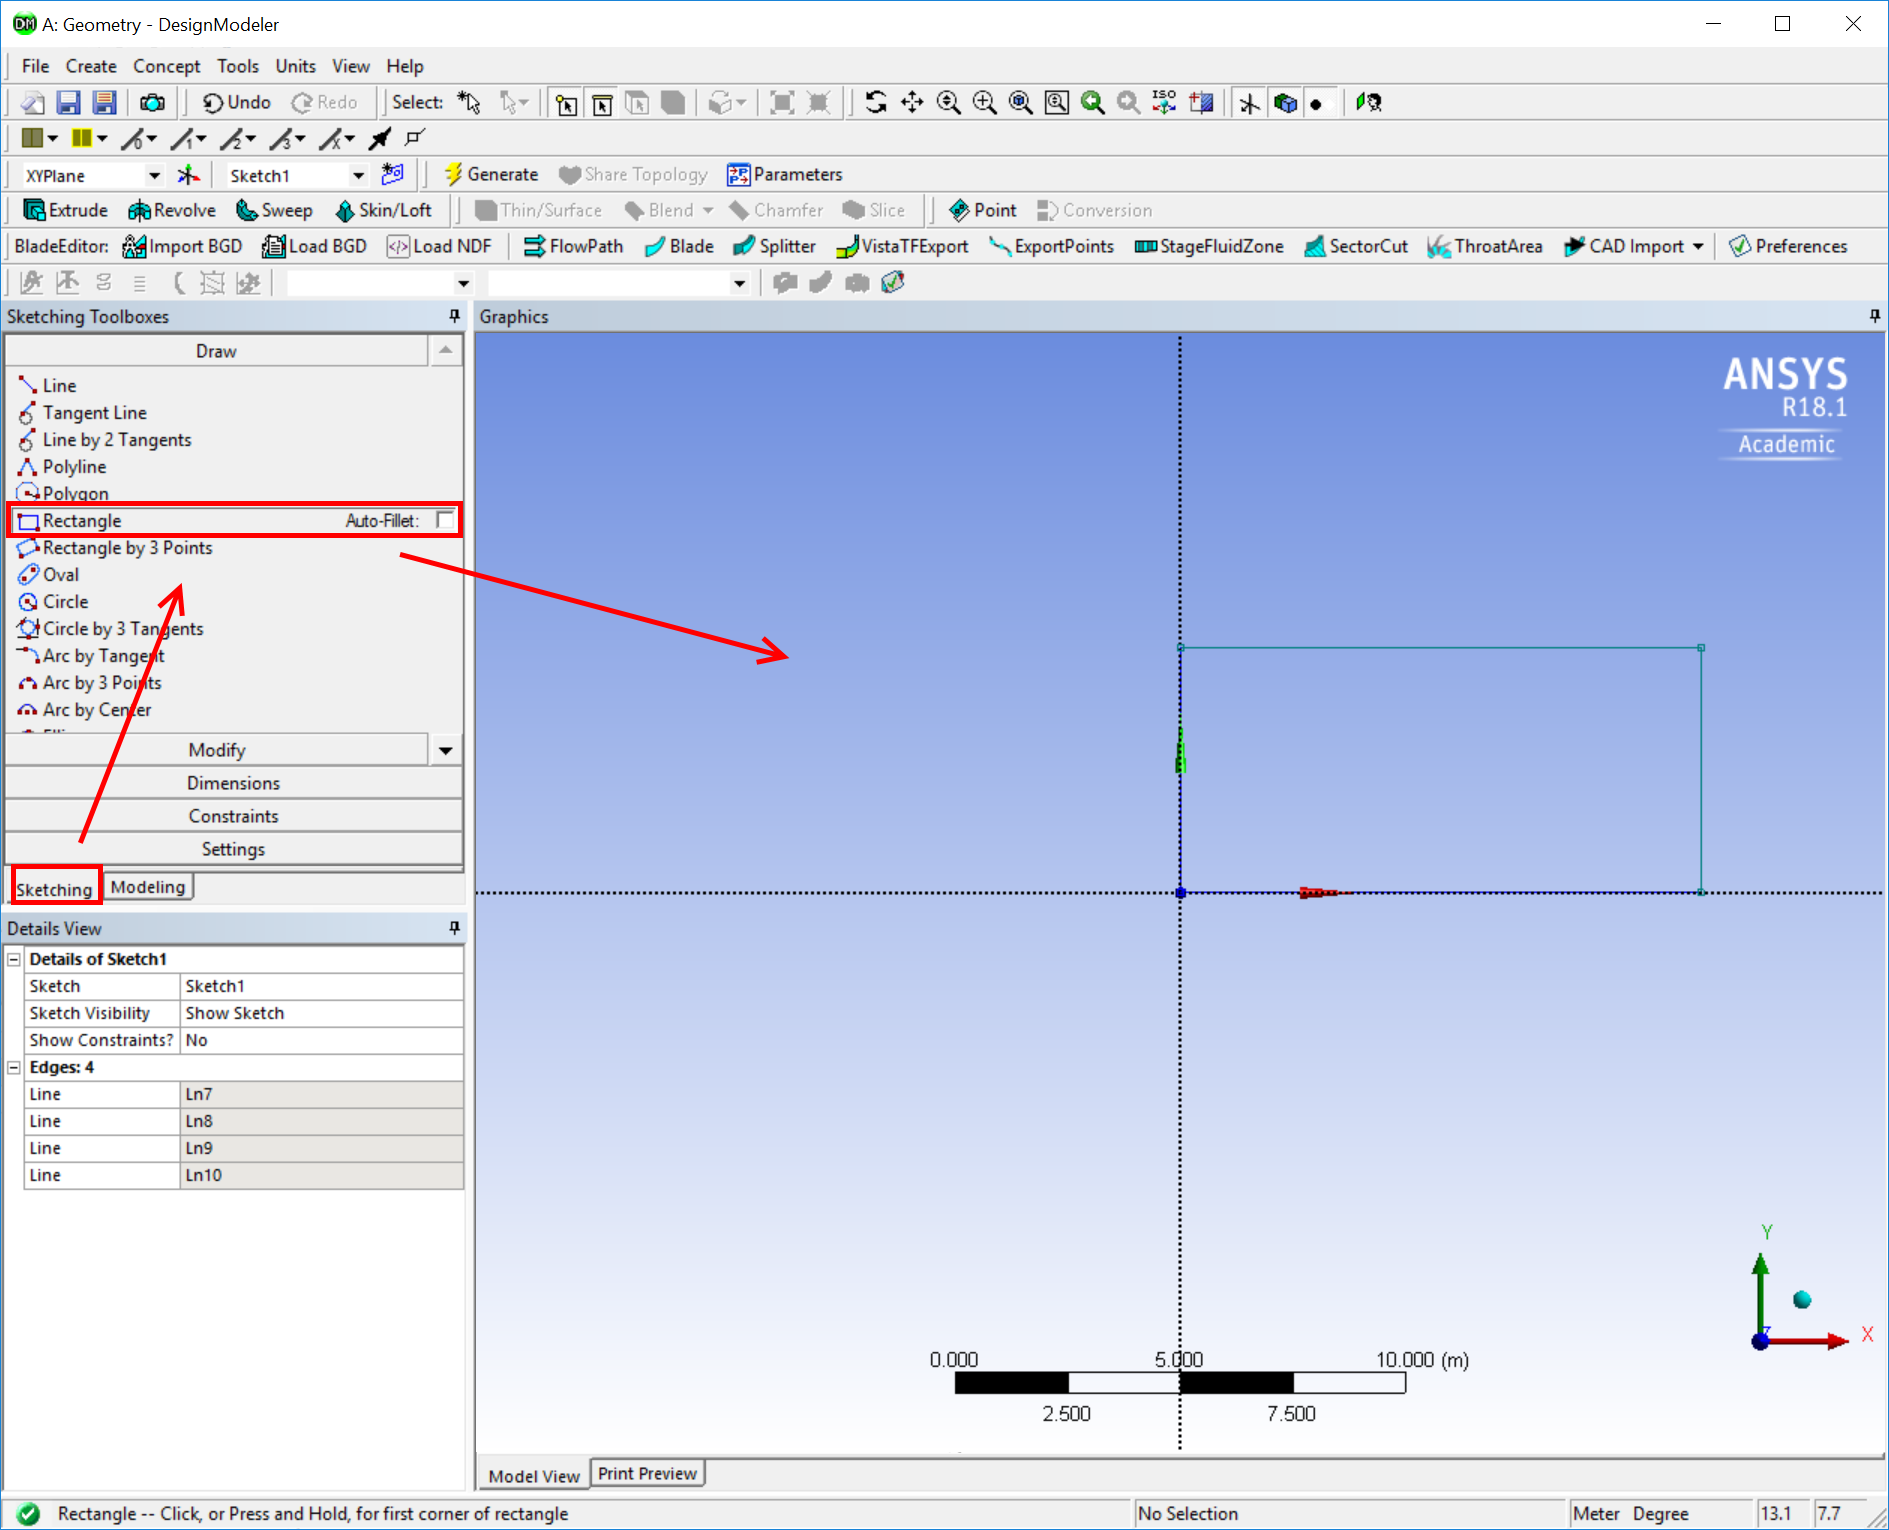
\includegraphics[width=0.7\textwidth,clip]{draw_rectangle.png}
\end{center}
\end{figure}

\subsubsection{Setting the dimensions}
Here we will set the dimensions of the rectangle, which only consist of a horizontal and vertical dimension. Select the \bfr{Dimensions} menu in the \bfr{Sketching tab} and select \bfr{Vertical}. In the \emph{Graphics Window} click once on the upper boundary of your rectangle and once on the lower boundary, then drag  ``V1'' outside the left side of the rectangle and click once more. Note, the label "V1"  denotes the "vertical1" where the number 1 indicates the sequence number in your dimensioning (so this would be 2 if you had decided to dimension the horizontal dimensions first). Repeat the procedure for the horizontal dimension by selecting \bfr{Horizontal} in the \bfr{Dimensions} menu and selecting the left and right boundaries of your rectangle.

\begin{figure}[H]
\begin{center}
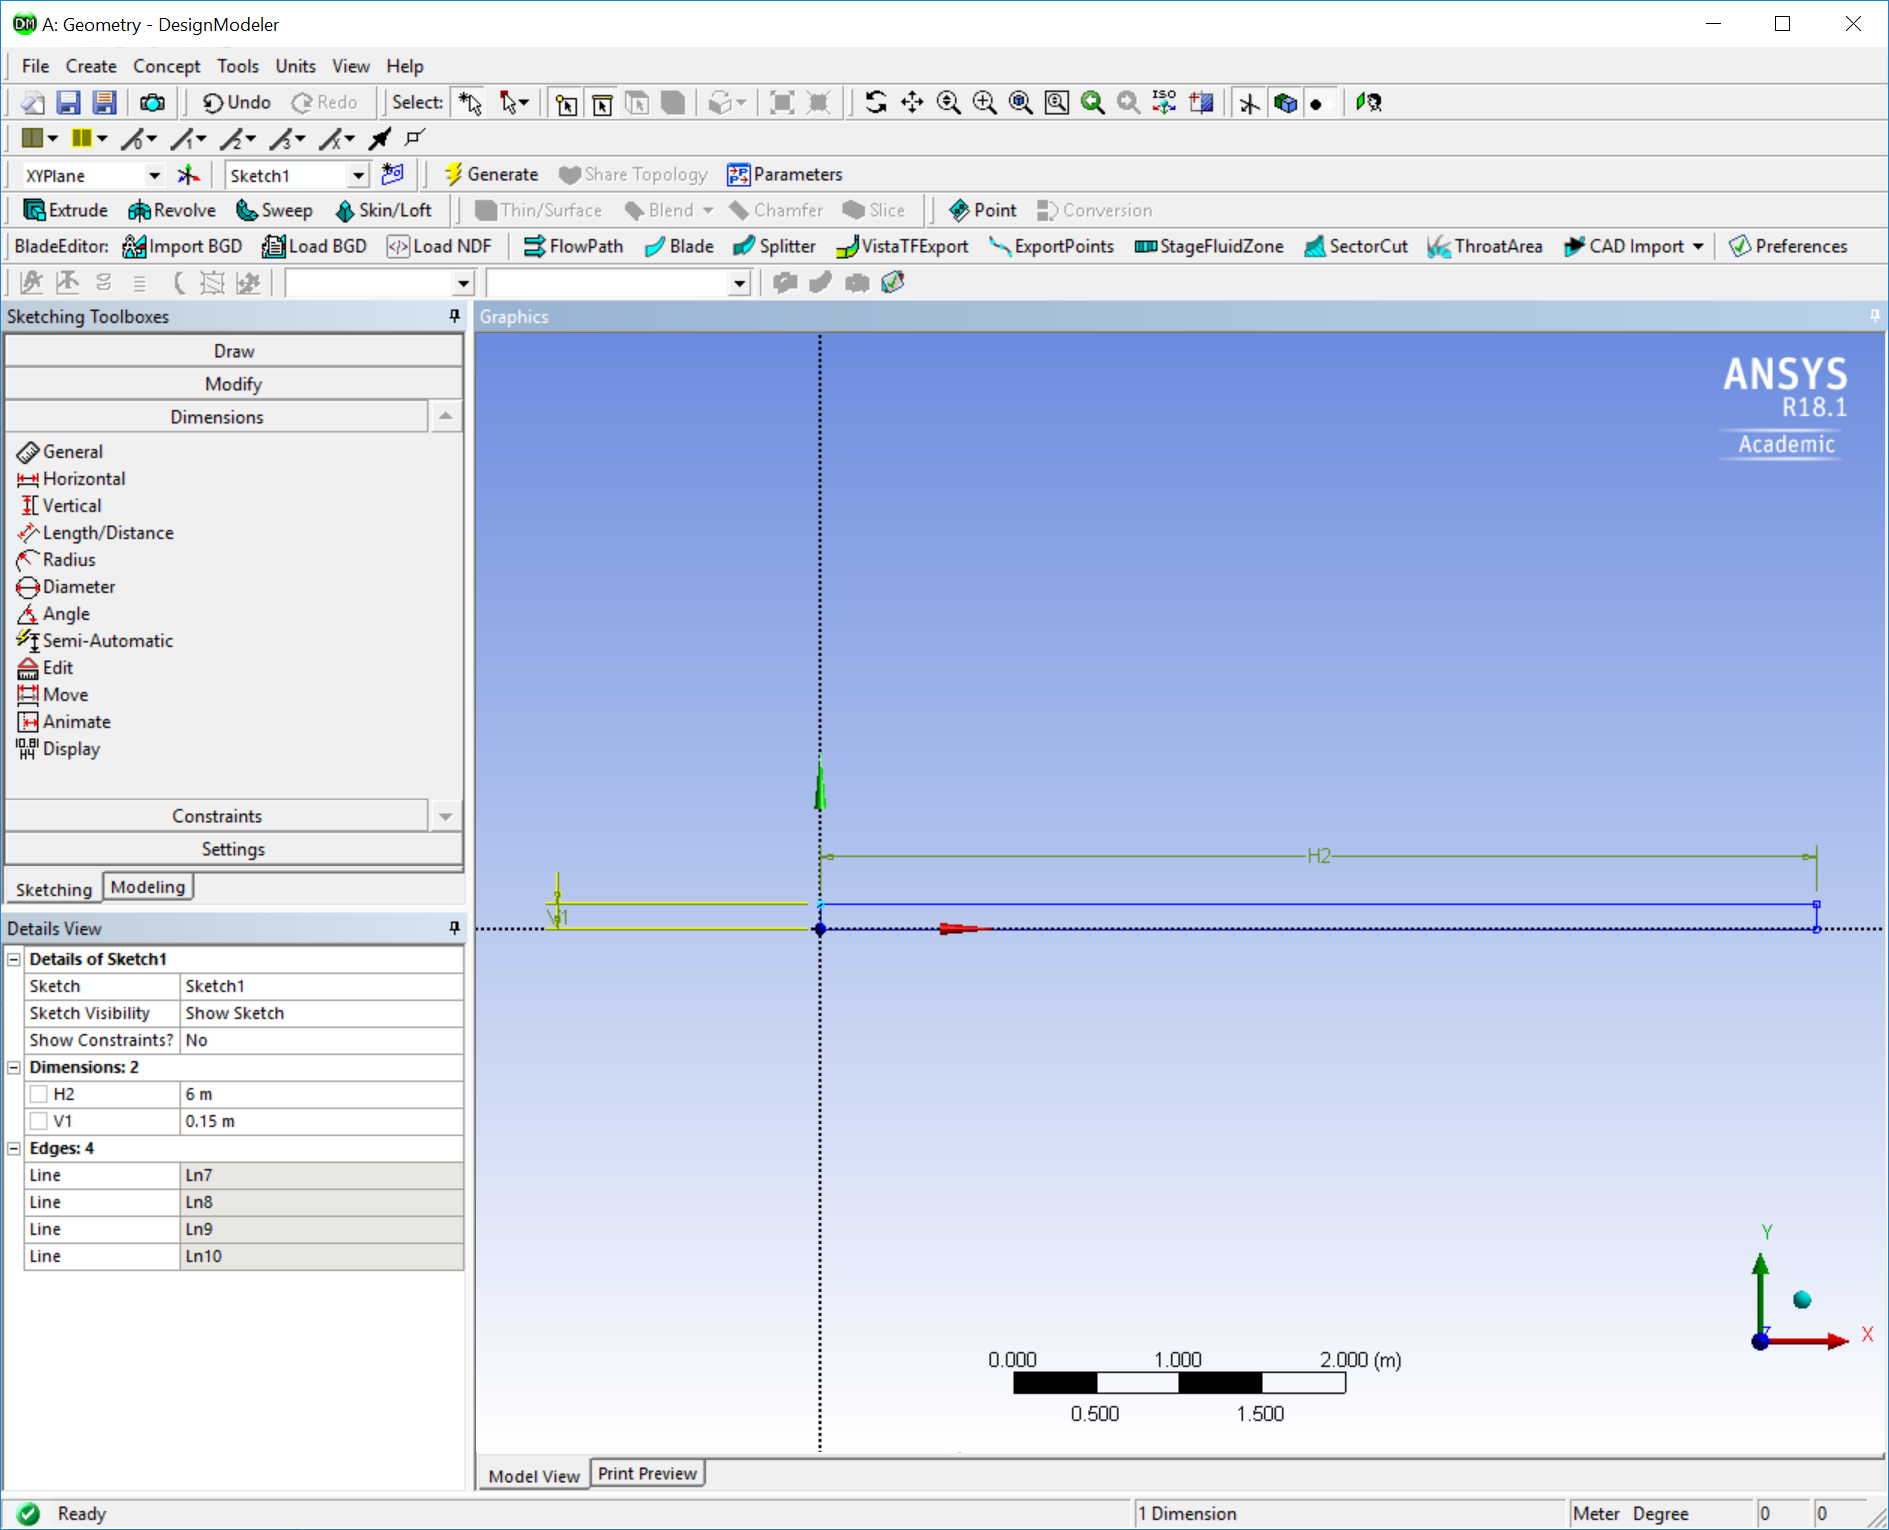
\includegraphics[width=0.7\textwidth,clip]{rectangle_dimensions.png}
\end{center}
\end{figure}

Set the dimensions in the \emph{Details View} table, located in the lower left corner. Remember that the flow is \emph{axisymmetric} therefore we only needed to model a plane of height $R=D/2=0.15\,$m, therefore V1=0.15\,m, and length $L=6$\,m, therefore H2=6\,m,


\subsubsection{Creating the surface}

Select the \bfr{Sketch1} in the modelling tab of the \emph{Tree Outline}, the four lines of your created rectangle should turn yellow. Now select \bfr{Concept} in the \emph{menu bar} and select \bfr{Surfaces from Sketches} as shown below.
\begin{figure}[H]
\begin{center}
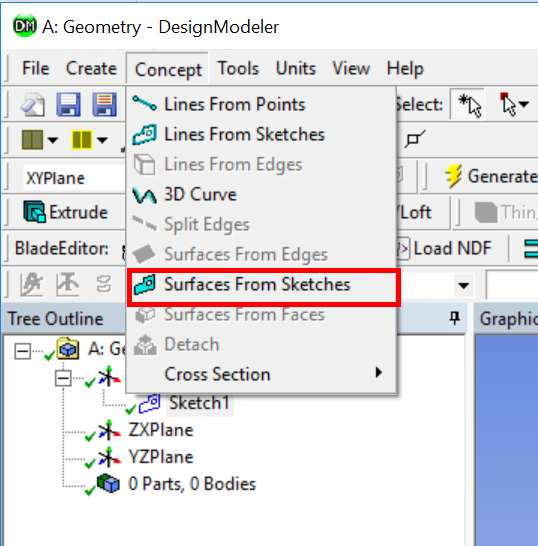
\includegraphics[width=0.3\textwidth,clip]{surfaces_from_sketches.png}
\end{center}
\end{figure}

Click \bfr{Apply} in the \emph{Details View} table in the lower left corner and click the 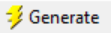
\includegraphics[width=1.2cm]{generate_button.png} button in the \emph{Feature Toolbar}. Your created geometry should now look as follows
\begin{figure}[H]
\begin{center}
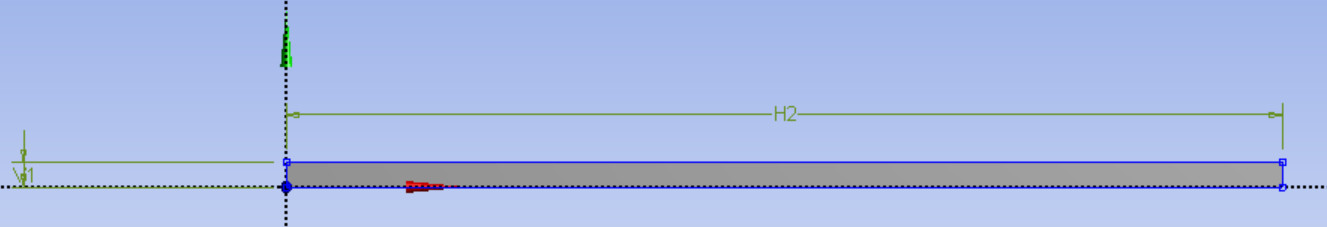
\includegraphics[width=0.7\textwidth,clip]{pipesurface.png}
\end{center}
\end{figure}

Now, we only need to tell the software that the surface we have created is part of the Fluid domain, and not the solid domain which it assumes by default. In the Tree Outline, select the ``+'' symbol next to \emph{1 Part, 1 Body} and select the \emph{Surface Body} that was created. In the details view below change the domain to \emph{Fluid} as shown below.

\begin{figure}[H]
\begin{center}
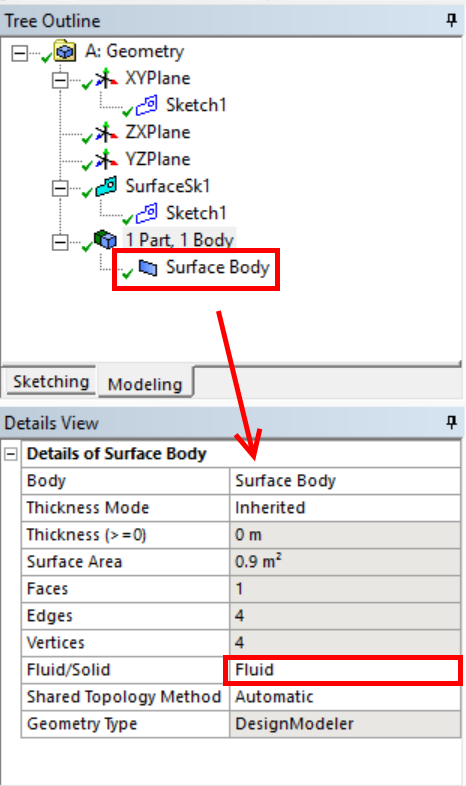
\includegraphics[width=0.25\textwidth,clip]{Fluid_domain.png}
\end{center}
\end{figure}

\subsubsection{Save the project}
Now that you have successfully created your pipe geometry you can close the \emph{DesignModeler} window and return to your \emph{Workbench} window. Note how a \cm  symbol has appeared in the Geometry cell, indicating that you have completed a geometry (if you only draw a single line the \cm  symbol would still have appeared, so it does not necessarily mean you have drawn an valid geometry!).

In the workbench you can save the project by clicking \bfr{Save} or \bfr{Save As..}, give your project a sensible name, e.g. LamPipeFlow and save it in your working directory on your \emph{Homedrive}. Note that not only the file \bfr{LamPipeFlow.wbpj}, is created within your working directory, but also the folder \bfr{LamePipeFlow\_files}. In order to open your project at a future occasion you will need both the \bfr{*.wbpj} file and the accompanying folder with its contents.

\subsection{Mesh generation}

\subsubsection{Launching the meshing window}

Drag the \bfr{Mesh} component from the \emph{Component Systems} menu to the \emph{Project Schematic}. Establish a link between the geometry and mesh, by dragging the \bfr{Geometry} cell from your Geometry component table, to \bfr{Geometry} in the Mesh component table. A line will be established between the two and the \cm symbol will appear next to Geometry in the Mesh component box. Now the Mesh needs to be made aware of the added geometry: right-click the \bfr{Mesh} cell and select \bfr{Refresh}, after about 5-10s the refreshing procedure is complete and a lightning bolt symbol will appear next to the Mesh.

\begin{figure}[H]
\begin{center}
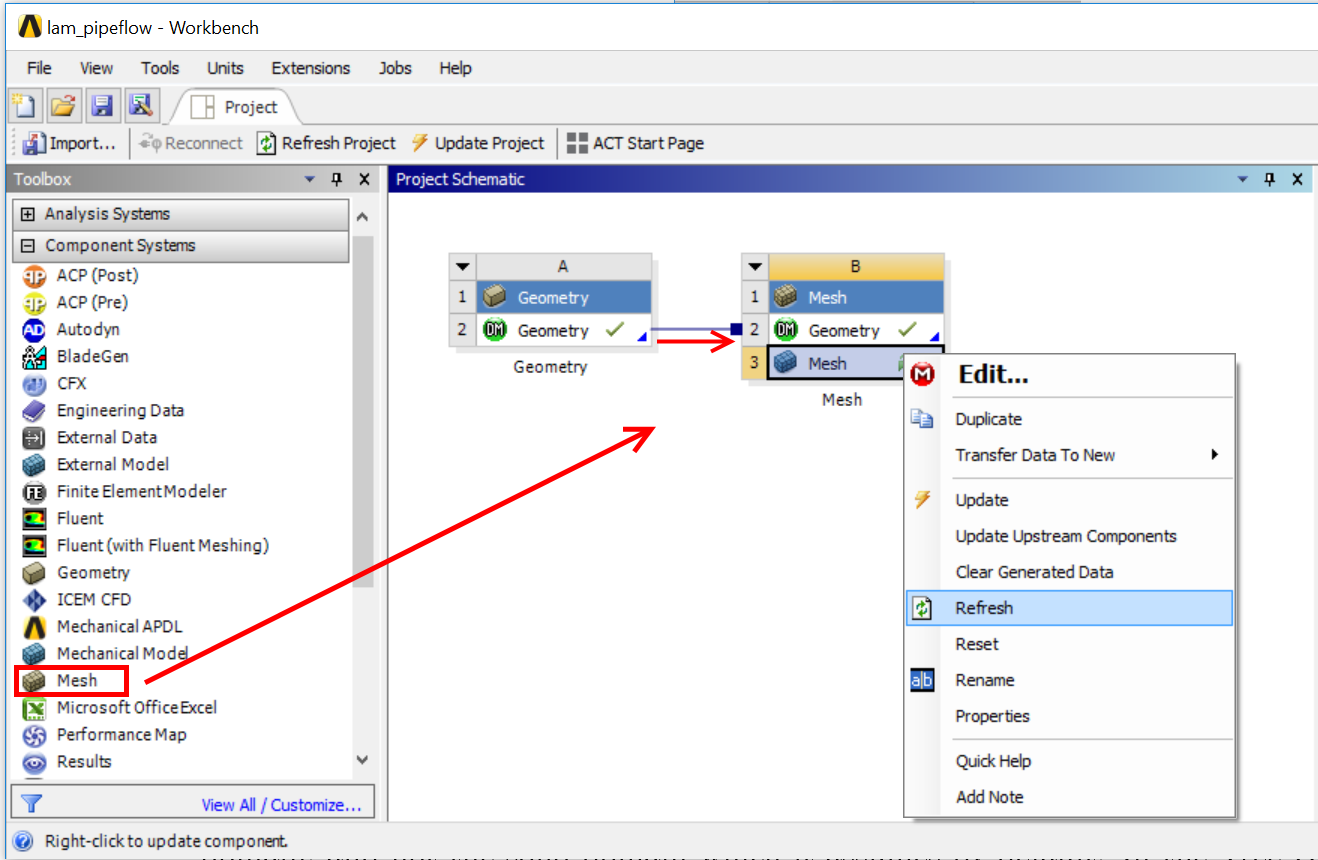
\includegraphics[width=0.7\textwidth,clip]{Mesh_workbench.png}
\end{center}
\end{figure}

Now right-click \bfr{Mesh} and select \bfr{Edit} (or double-click \bfr{Mesh}), this will open the \emph{Meshing} window. The outline of this window is similar to the \emph{DesignModeller} window which you used to create your geometry, ie. on top you see the various \emph{toolboxes}, in the upper left column you see your project's \emph{Tree Outline}, where you can select different components of your model, in the lower left column you see \emph{Details View} table of the selected component, and the main window contains your \emph{Geometry Window}. Below the geometry you will now also see a \emph{messages} window which displays any error messages that might result from your actions.

\subsubsection{Creating named selection}

Before we generate the mesh we will first give names to the four edges of our geometry. This will allow us to recognise the edges more easily and assign boundary conditions in the Fluent solver later on.

Click the edge tool symbol 
\includegraphics[width=0.5cm]{edge_tool.png} in the \emph{selection toolbar} and click on the left edge of your geometry in the \emph{Geometry Window}. Right-click on the green highlighted line and select \bfr{Create Named Selection} as shown below. Note that you can zoom in and change the view of your geometry using the various magnifying glass tools in the \emph{rotation mode toolbar} at the top of your window. To restore the view of your entire geometry click the zoom to fit symbol 
\includegraphics[width=0.5cm]{zoom_to_fit.png}.

\begin{figure}[H]
\begin{center}
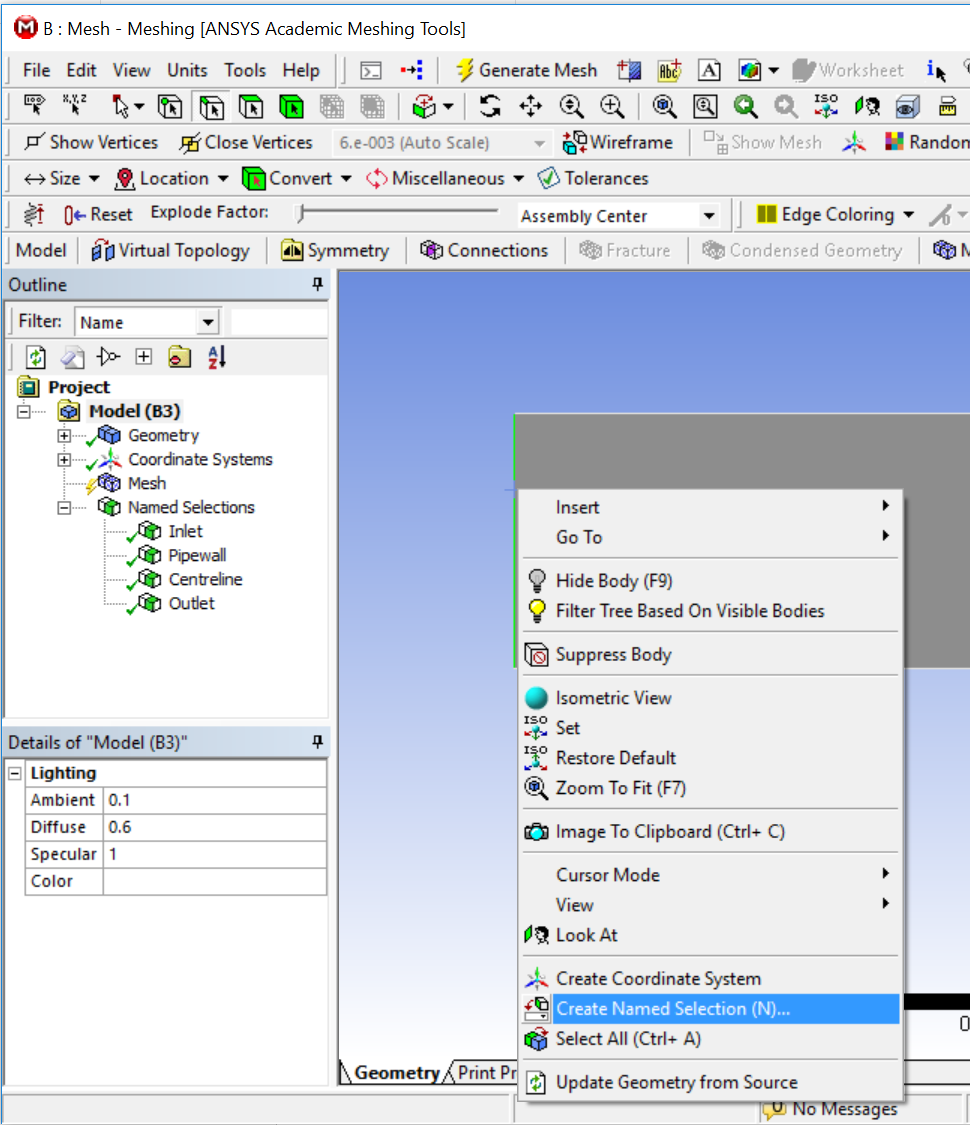
\includegraphics[width=0.6\textwidth,clip]{create_named_selection.png}
\end{center}
\end{figure}

Give the boundary the name \bfr{Inlet} in the Selection name window that appears. Repeat the procedure to name the upper (\bfr{Pipewall}), right (\bfr{Outlet}) and lower (\bfr{Centreline}) boundaries. Your four named boundaries should now have appeared under the \bfr{Named Selections} item in the \emph{Tree Outline}. Finally, we are also going to name the interior part of our domain: click on the \emph{named selection} in the Project Tree and then choose the face select tool 
\includegraphics[width=0.5cm]{face_tool.png}, click on the gemoetry such that it highlights green, now you can rightclick on the surface and rename it to \emph{flow\_domain}.


You can display the named selections in your geometry by changing the \bfr{Show Annotations} to ``yes'' in the \emph{Details View} table as shown below.

\begin{figure}[H]
\begin{center}
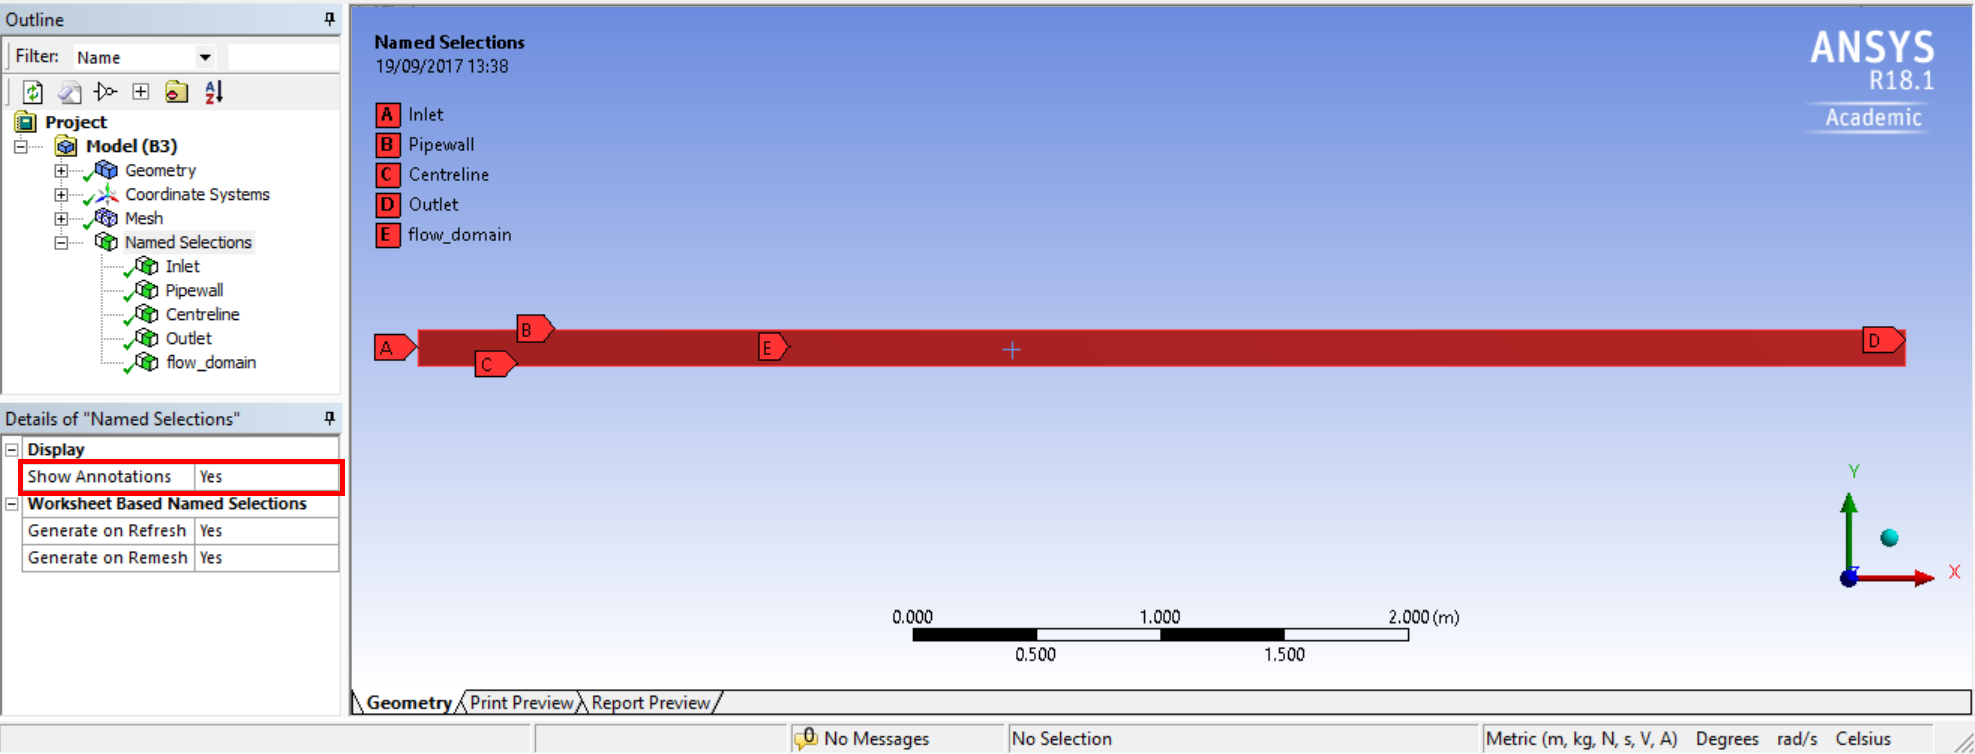
\includegraphics[width=0.7\textwidth,clip]{named_selections.png}
\end{center}
\end{figure}


\subsubsection{Creating uniform structured Mesh}
Here we are going to create a \emph{structured} or grid style mesh on a selected face, in this case our pipe. Right-click \bfr{Mesh} in the \emph{Tree Outline}, select \bfr{Insert} and then select \bfr{Face Meshing} from the drop-down menu, as shown below (alternatively, you can select \bfr{Face Meshing} from the \bfr{Mesh Control} toolbar indicated below).

\begin{figure}[H]
\begin{center}
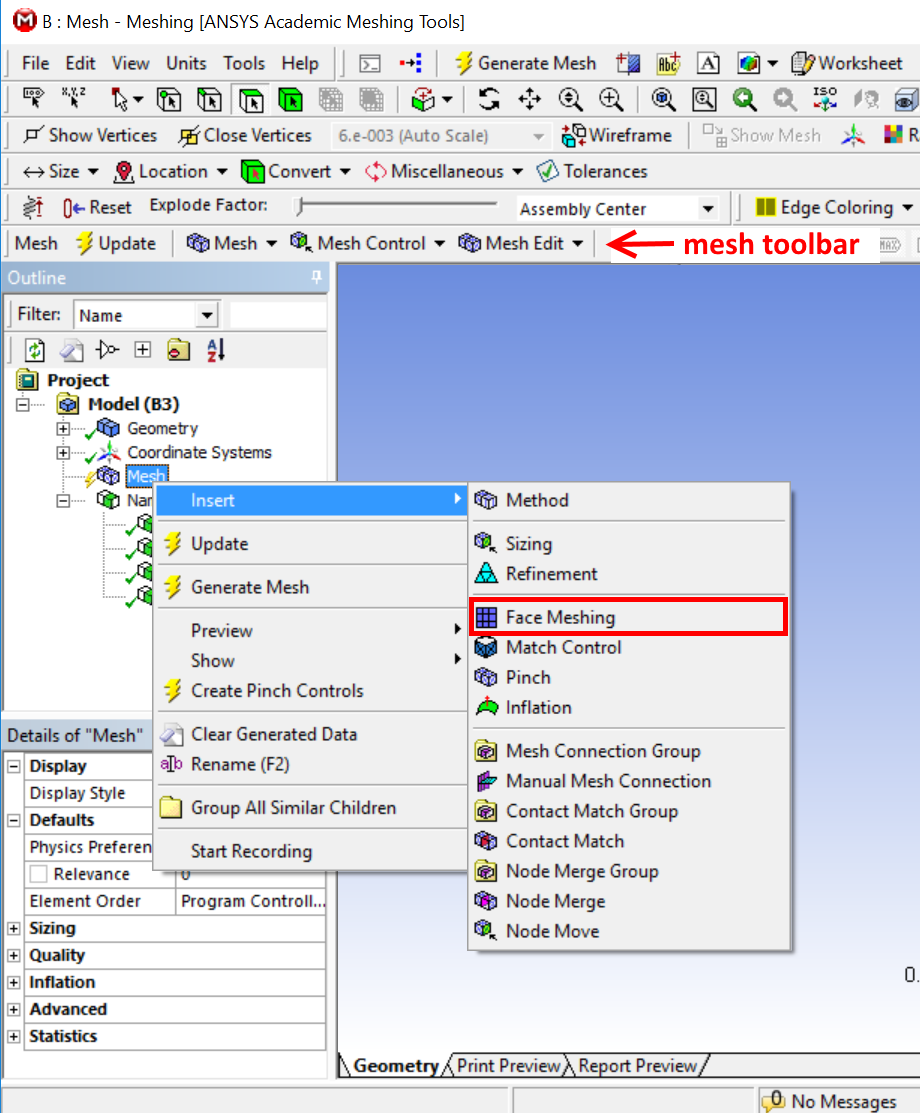
\includegraphics[width=0.4\textwidth,clip]{face_meshing.png}
\end{center}
\end{figure}

After clicking face meshing you will see in the \emph{Details View} that the Geometry box is highlighted in yellow and indicates ``No selection'', this means that we still have indicate to which surface we need to apply the Face Mesh. In our case the Geometry will be the pipe surface, so therefore click on the pipe face in the Geometry Window, the surface should should highlight green. Now go to the \emph{Details View} of the face meshing menu and click on \bfr{no selection} in the yellow Geometry cell, then click \bfr{Apply}. The Geometry cell should now list \bfr{1 Face} and our pipe surface selected face should have turned blue in colour.

\begin{figure}[H]
\begin{center}
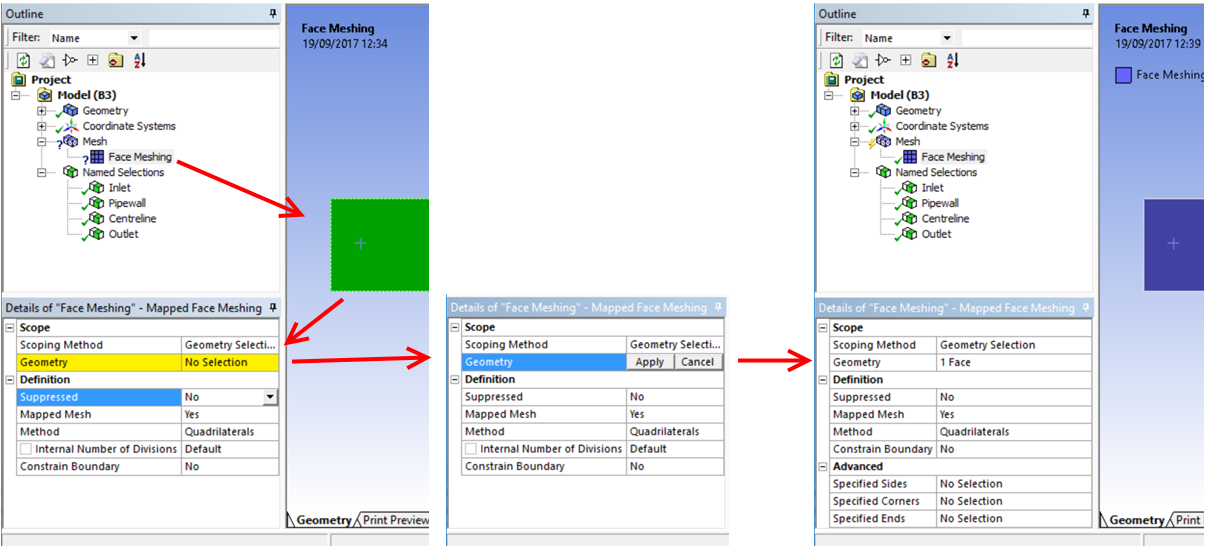
\includegraphics[width=0.85\textwidth,clip]{apply_mfm.png}
\end{center}
\end{figure}
We are almost there. You still need to generate the mesh:  right-click \bfr{Mesh} in the \emph{Tree Outline}, and select \bfr{Generate Mesh}. Great, we have now created our default mesh, which can be seen if you select \bfr{Mesh} in the Tree Outline. The mesh should look as follows:
\begin{figure}[H]
\begin{center}
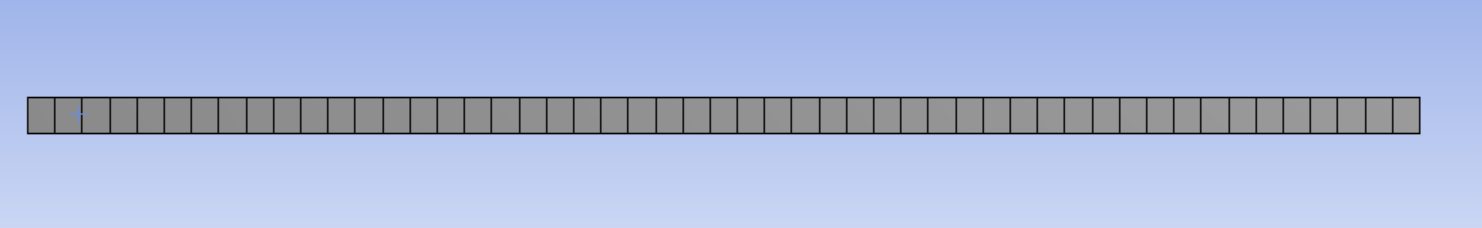
\includegraphics[width=0.7\textwidth,clip]{default_mesh.png}
\end{center}
\end{figure}


\subsubsection{Edge sizing}

Our default mesh only consists of 51 elements (this can be seen in the \emph{Details View} of ``Mesh'' by double-clicking on statistics \emph{Statistics}). This is rather coarse mesh, in particular in the vertical (radial) direction we only have one cell. There we are going to increase the mesh to 600 elements, 8 in the vertical and 75 in the horizontal. We can achieve this by specifying the number of divisions on the edges of our geometry. We will start by specifying the number of divisions at the Pipewall and the Centreline. Click \bfr{Mesh Control} in the \emph{mesh toolbar} and select \bfr{Sizing} from the drop-down menu:
\begin{figure}[H]
\begin{center}
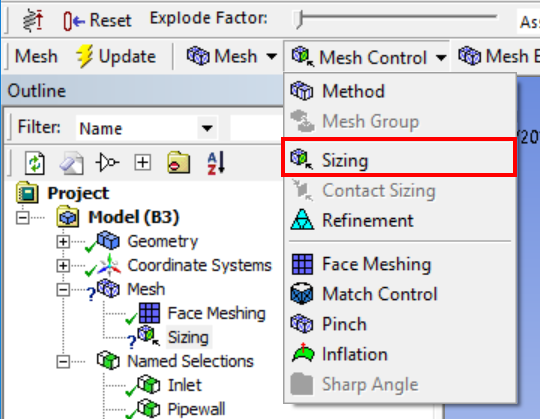
\includegraphics[width=0.4\textwidth,clip]{mesh_sizing.png}
\end{center}
\end{figure}
Now, make sure that you have the edge tool 
\includegraphics[width=0.5cm]{edge_tool.png} selected, then hold down the Ctrl-key and select the top and bottom edge of your geometry, which should highlight green, then click \bfr{Apply} in the \emph{Details View} table as follows:
\begin{figure}[H]
\begin{center}
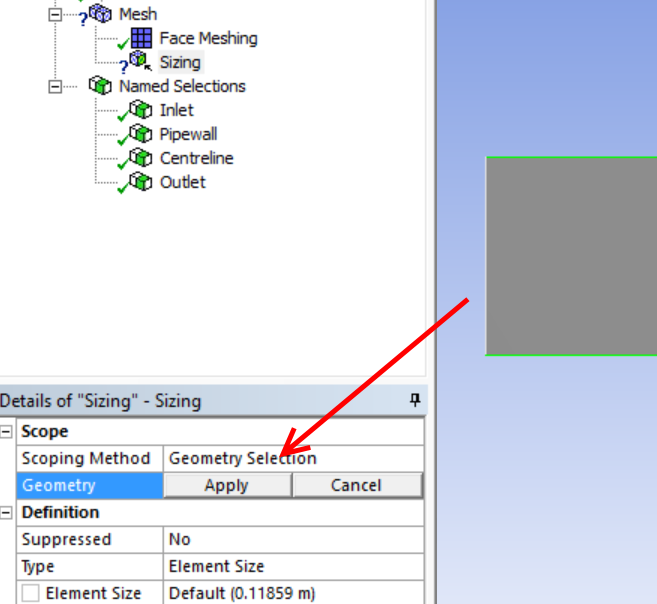
\includegraphics[width=0.4\textwidth,clip]{apply_edge_sizing.png}
\end{center}
\end{figure}
Change the cells in the Details View table as follows:
\begin{figure}[H]
\begin{center}
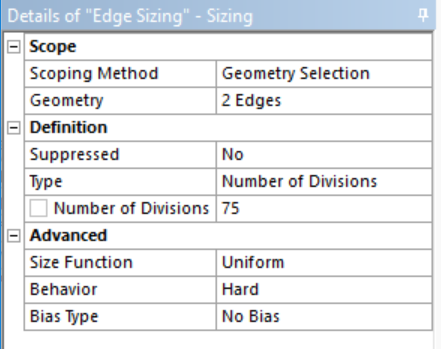
\includegraphics[width=0.3\textwidth,clip]{Details_of_sizing.png}
\end{center}
\end{figure}
Click the update button 
\includegraphics[width=1.cm]{update_button.png} in the \emph{mesh toolbar} to update your mesh. Now repeat the process to apply 8 divisions to the left (inlet) and right (outlet) boundaries of your pipe.
\\
\\
Select \bfr{Mesh} in the \emph{Tree Outline} to view your created mesh, which should look as below. Verify in the \bfr{Details of Mesh} table that your mesh contains the required 600 elements. (Note that by changing the sizing behaviour from \emph{soft} to \emph{hard} has forced the divisions along an edge to be of equal size. At this stage you can check yourself what effect the behaviour setting has on your mesh ).


\begin{figure}[H]
\begin{center}
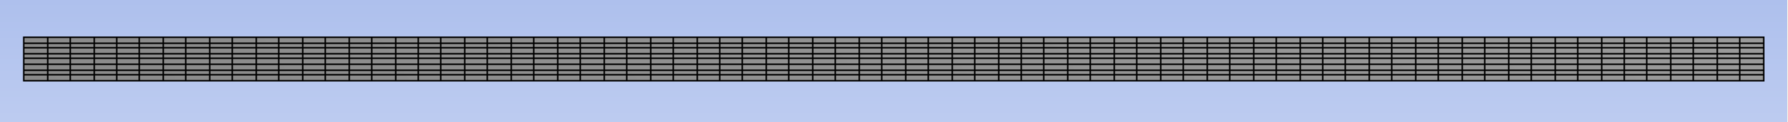
\includegraphics[width=1.0\textwidth,clip]{laminar_mesh.png}
\end{center}
\end{figure}

Save your project and close the \emph{Meshing} window, then in your \emph{Workbench} click the 
\includegraphics[width=1.5cm]{update_project.png} button and make sure to save your project once more.

\FloatBarrier

\subsection{FLUENT analysis}
Now, we are at the third stage, the Fluent Solver. This aspect contains of two main steps: 1. setting-up our mathematical model and 2. specifying how we are going to solve our mathematical model.
In the first step we need to specify the governing equations and boundary conditions for our problem and while in the second step we specify which discretization methods we are going to use when solving the equations.

In the \emph{Workbench} drag the \bfr{Fluent} component system to the \emph{project schematic} and then drag the \bfr{Mesh} cell from the mesh component table to the \bfr{Setup} cell of your Fluent component table. This action might cause a 
\includegraphics[width=.4cm]{lightning_symbol.png} symbol to appear next to you previously generated mesh, if so, right-click on the mesh and select \bfr{Update}. Now, right-click on \bfr{Setup} in the fluent component and select \bfr{Refresh} from the drop-down menu.

\begin{figure}[H]
\begin{center}
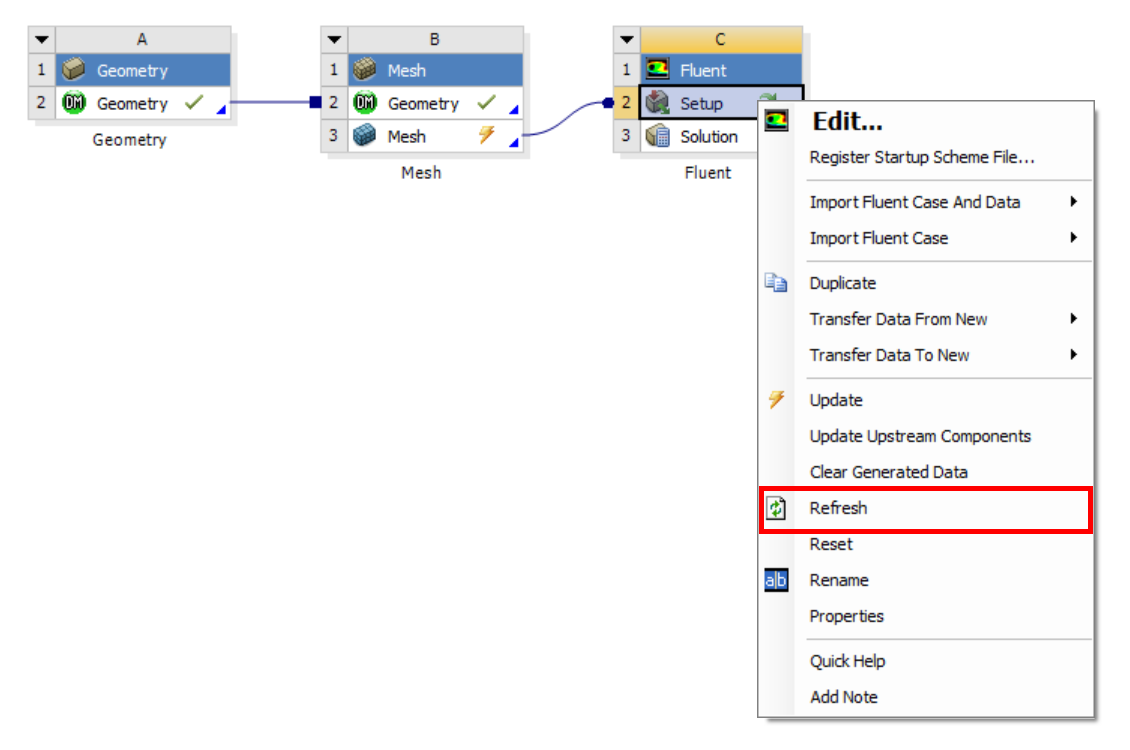
\includegraphics[width=0.7\textwidth,clip]{fluent_workbench_refresh.png}
\end{center}
\end{figure}
Double-click \bfr{Setup} (or right click and press Edit), then change the options to \bfr{Double Precision} in the Fluent Launcher window that appears, then select \bfr{OK}.
\begin{figure}[H]
\begin{center}
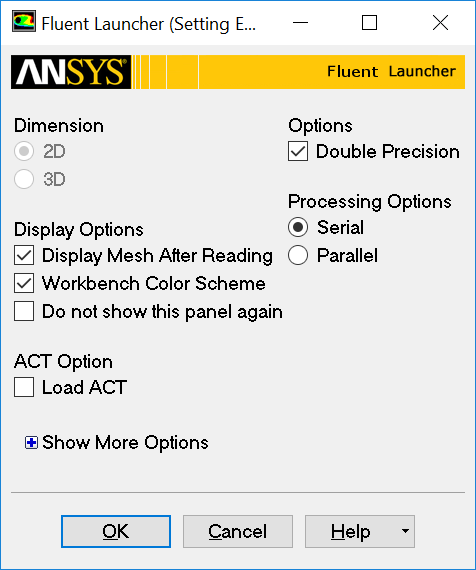
\includegraphics[width=0.3\textwidth,clip]{fluent_launcher.png}
\end{center}
\end{figure}
After a while, the Fluent interface will show up, which consists of the areas shown below. As before we will use these terms to guide you through the process.
\begin{figure}[H]
\begin{center}
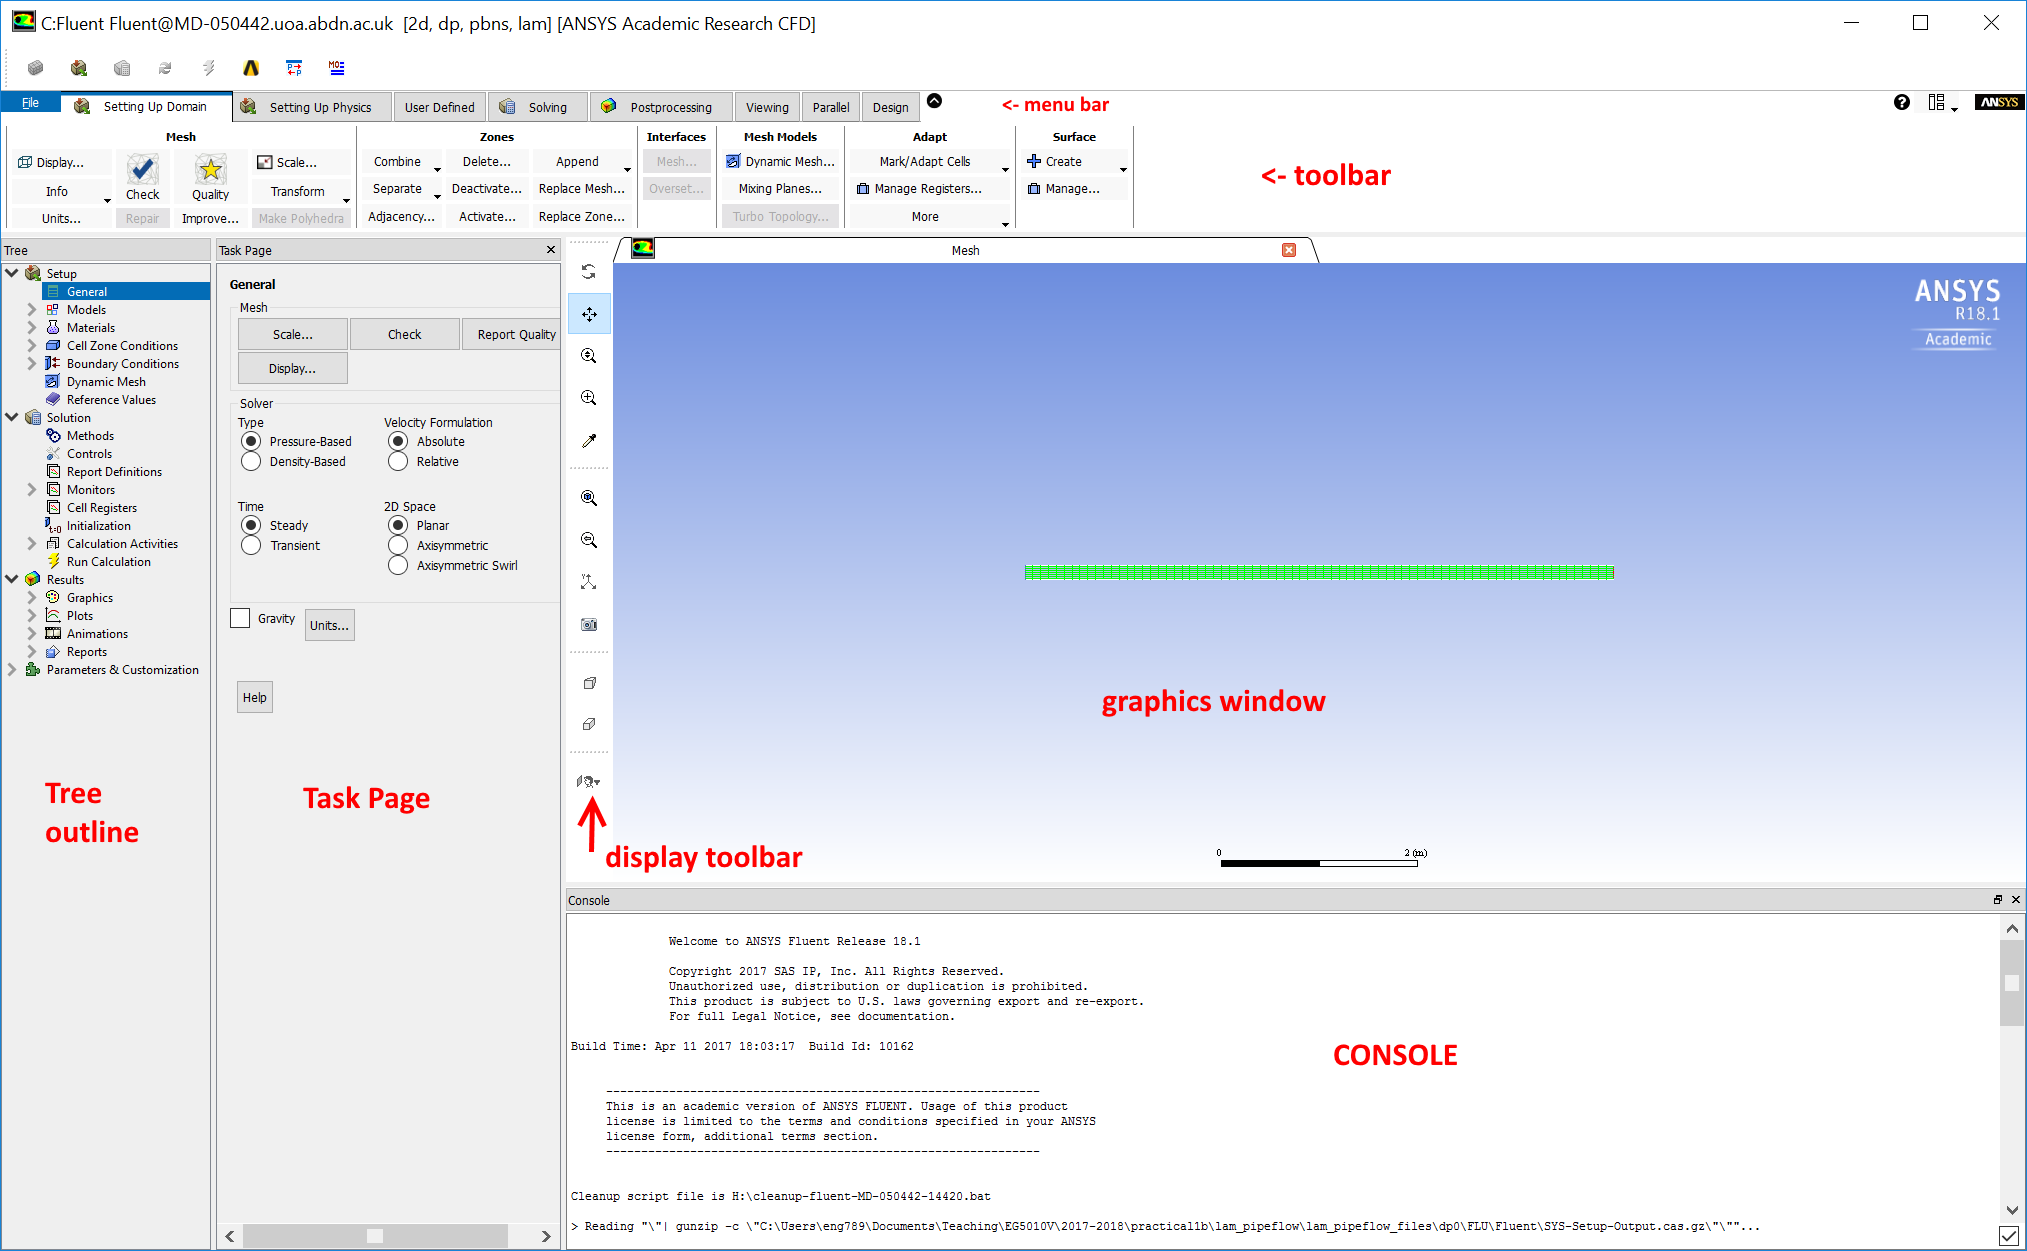
\includegraphics[width=0.7\textwidth,clip]{Fluent_GUI.png}
\end{center}
\end{figure}

In the \emph{Project Tree} you can see the two main components discussed above, the first is \emph{Setup} in which we define our mathematical models and \emph{Solution} under which we going to specify how we are going to solve the mathematical model.
In the Fluent analysis we will essentially work our way through the items in the \emph{Project Tree} from the top until \emph{run calculation}. The activities can be grouped as follows:\\

\emph{Perform pre-analysis checks:}
\begin{enumerate}[nolistsep]
    \item	Solving any warning messages.
    \item	Mesh checking.
\end{enumerate}
\emph{Setting up the mathematical model:}
\begin{enumerate}[resume,nolistsep]
    \item	Select Model and material properties
    \item	Setting up the boundary conditions.
\end{enumerate}
\emph{Specify how to solve the model:}
\begin{enumerate}[resume,nolistsep]
    \item   Setting up the solution methods and controls.
    \item	Monitoring solution convergence.
\end{enumerate}
\emph{Perform the calculation:}
\begin{enumerate}[resume,nolistsep]
    \item	Initializing the simulation.
    \item	Running the calculation
\end{enumerate}

In the following section we will go through these activities. Note that analysis (i.e. \emph{post-processing}) of the results will be addressed separately in Section~\ref{sec:postproc}.

\subsubsection{Checking warning messages}
It is good practice to scroll through the Console window and check if there any warning messages displayed. If you have followed all the steps correctly so far there will not be any warning messages displayed. However, if you do see warning messages at this stage than you will have made an error in the geometry or meshing stages. The warning message will give a description of the error which you will first need to correct before proceeding in the Fluent solver.

\subsubsection{Check Mesh and Display}
In this step we are going to check whether the mesh is correctly imported into the fluent solver. The first step before we are going to perform this check is telling Fluent that the model is an \emph{axisymmetric}: click \bfr{General} in the \emph{Navigation Pane} and then in the \emph{Task Page} select \bfr{Axisymmetric} under 2D space. In the Mesh menu select select \bfr{Check}, the console should now display the following:
\begin{figure}[H]
\begin{center}
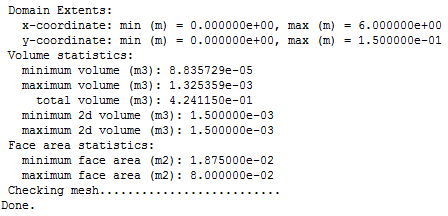
\includegraphics[width=0.35\textwidth,clip]{mesh_check_commandpane.png}
\end{center}
\end{figure}

If console displays \emph{Done} after the mesh checking than your mesh is approved. If it indicates errors than you will need to go back to the meshing stage and correct the errors. More information can be obtained from the Mesh Info buttom which you can find in the toolbar. The Size Info will display information on the number of Cells (elements) which we have previously set 600.

Click \bfr{Display} in the \emph{Task Page} or in the \emph{Toolbar}. In the Mesh Display dialog box that appears note that under Surfaces our four named boundaries are listed, and the (interior) fluid domain. Select all five surface and click the \bfr{Display} button. Note how your mesh is displayed in the Graphics Window. Use the various tools from the Graphics Toolbar to investigate the mesh in more detail, remember that you can restore the full view by clicking 
\includegraphics[width=.5cm]{zoom_to_fit.png} in the display toolbar. \bfr{Close} the Mesh Display dialog box.


\subsubsection{Select Model and material properties}
In this section we will essentially tell Fluent which are the governing equations that need to be solved. In any fluid flow problem we will solve the \emph{continuity equation} and the \emph{momentum equation}, these you therefore do not have to select in Fluent. However, you do have to tell Fluent which type of the momentum equation you will solve, i.e. whether it is for inviscid flow, laminar flow or for turbulent flow. In our case the flow is laminar which we can specify by selecting under \bfr{Models} in the \emph{Navigation Pane}. Note how the \emph{Task Page} will display a list of models, in this case we only have to set the \bfr{Viscous} model. Select the \bfr{Viscous} model and click \bfr{Edit}. The Viscous Model dialog box will show a of the various ways in which we can solve the momentum equation in Fluent, besides the inviscid and laminar models this list contains various types which can be used to solve turbulent flow (\hl{lec} and the next tutorial). We are dealing with laminar flow in this problem so for now leave the viscous model selected at \bfr{Laminar}, click \bfr{OK} to exit the dialog box. Ensure that all the other models (Multiphase, Energy, etc.) are switched off, these are not part of our flow problem.

The next step is tell Fluent what type of fluid we are dealing with, because the density and viscosity of the fluid appear in the governing equations.
First of we need to create our fluid: click on \bfr{Materials} in the \emph{Tree Outline} and then right click on  \bfr{Fluid} and select \bfr{New}.  In the dialog box that appears you can enter the density and viscosity of the fluid.  Note there is also a button \emph{Fluent database} in this dialog box, this allows you to pick a fluid from a vast database incorporated in Fluent. In this case we are going to manually enter our fluid properties, so change the properties to our working fluid ($\rho=1.0$\,kg/m$^3$ and $\mu=1.5\times10^{-3}$\,kg/ms). Click \bfr{Change/Create} to close the window (note that the new fluid is named by default \emph{fluid-1} - you can change this name if you like). Under \emph{Fluid} in the \emph{Tree Outline} you will now find your newly created fluid named \emph{fluid-1}.

\begin{figure}[H]
\begin{center}
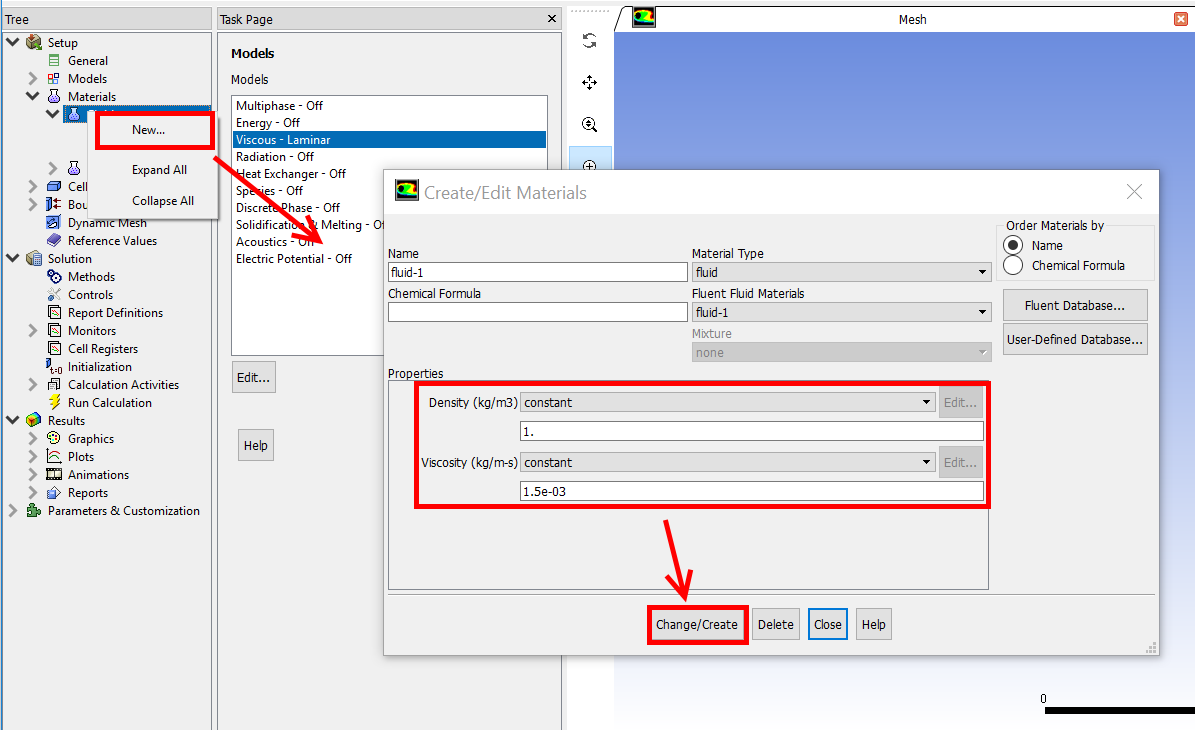
\includegraphics[width=0.7\textwidth,clip]{fluid_properties.png}
\end{center}
\end{figure}

Now we that we have created our fluid we still need to assign it to our fluid domain as follows, under \bfr{Cell Zone Conditions} in the \emph{Project Tree} double-click on the \bfr{flow\_domain}. In the dialog box that appears select our newly created \emph{fluid-1} under \bfr{Material Name} and select \bfr{OK}.
 \begin{figure}[H]
\begin{center}
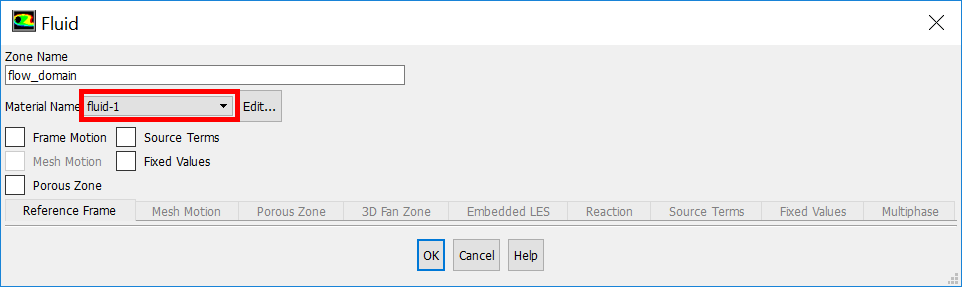
\includegraphics[width=0.7\textwidth,clip]{apply_new_fluid.png}
\end{center}
\end{figure}


\subsubsection{Boundary Conditions}

Here we are going to specify our boundary conditions. We have four boundaries to our domain (inlet, outlet, pipewall and centreline) so we have to set 4 boundary conditions (\hl{refer to fig 1 for b.c.'s??}):

\begin{enumerate}
\item \emph{inlet}: double-click \bfr{Boundary condition} in the \emph{Project Tree}, select \bfr{inlet} in the Task Page. In the bottom of the Task Page you can see under \emph{Type} that Fluent has already correctly guessed that the Type of boundary conditions is \emph{velocity-inlet} boundary condition. There are many more types of boundary conditions, but Fluent has made this guess (correctly) because we have named the boundary Inlet. Now click \bfr{Edit}, this will display the velocity inlet dialog box. Set the \bfr{Velocity Specification Method} to \bfr{Components} and set the \bfr{Axial Velocity} to 1 m/s as shown below, then click \bfr{OK} to close the velocity inlet dialog box.
\begin{figure}[H]
\begin{center}
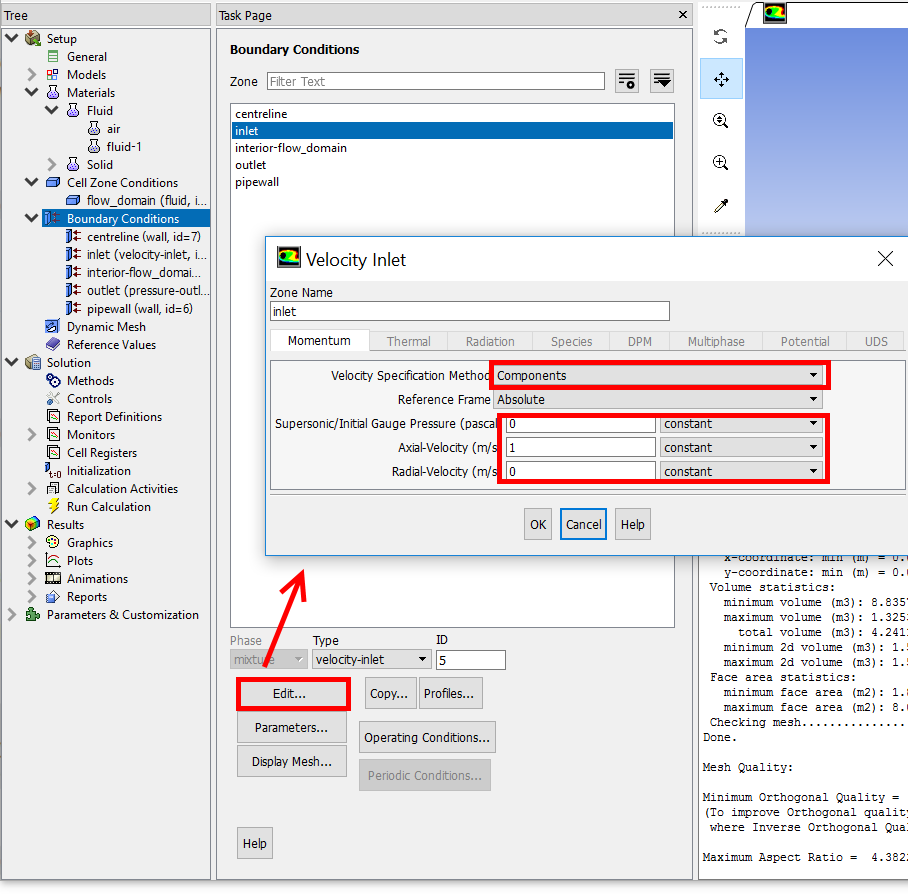
\includegraphics[width=0.7\textwidth,clip]{BC_velocity_inlet.png}
\end{center}
\end{figure}

\item \emph{outlet}: \hl{explain how fluent works with gauge pressure rather than absolute pressure}. Before we are going to specify the outlet boundary condition we are first going to set the operating pressure. Select \bfr{Operating Conditions}, in the dialog box that appears you will see that the operating pressure is set to 1\,atm (101325\,Pa), therefore leave this setting as it is and click \emph{OK}. Now select \bfr{outlet} in the boundary conditions task page and check if the \bfr{Type} is automatically set to \bfr{pressure-outlet} (this should be the case, but if it is not, change the type to pressure-outlet!). No further changes are needed since the gauge pressure by default is set to 0 Pascals (you can verify this by clicking Edit).
\item \emph{pipewall}: select the \bfr{pipewall} in the boundary conditions task page and verify that the \bfr{Type} is set to \bfr{wall}, if it is not then change it to \bfr{wall}. Click \emph{edit} and verify that the \emph{wall motion} is set to a stationary wall (our pipewall is stationary) and the \emph{shear condition} is set to No Slip (which means zero velocity at the wall). Click \bfr{OK} to close the dialog box.
\item \emph{centreline}: select the \bfr{centreline} from the boundary conditions task pane. You will notice that the \bfr{Type} is set to wall by default. This is incorrect guess by Fluent, because we want Fluent to treat it as an axis of symmetry, therefore change the type to \bfr{axis}. Click \bfr{OK} in any of the dialog boxes that appear.
    \begin{figure}[H]
    \begin{center}
    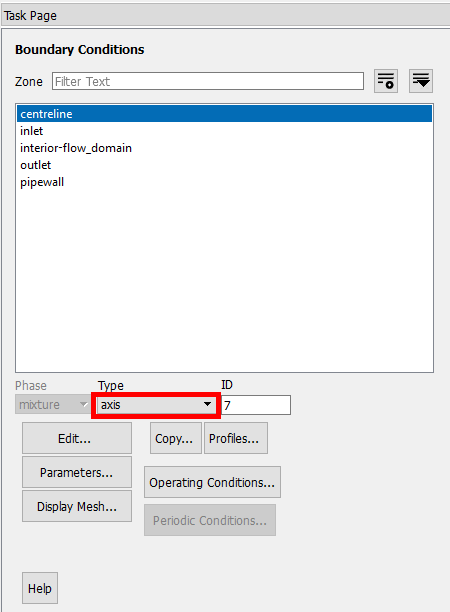
\includegraphics[width=0.4\textwidth,clip]{BC_centreline.png}
    \end{center}
    \end{figure}
\end{enumerate}


\subsubsection{Solution Methods and Controls}

The solution methods and controls refer to how the governing equations are discretisized (Lecture Notes 3). Here we will use the 2$^\mathrm{nd}$ order spatial discretization to solve our momentum equation. Select \bfr{Solution Methods} from the \emph{Project Tree} and verify that the settings are as follows. The other settings we are leaving our settings at their default values, however by checking the other options in the drop-down menus you can verify that Fluent contains many solution methods!
\begin{figure}[H]
\begin{center}
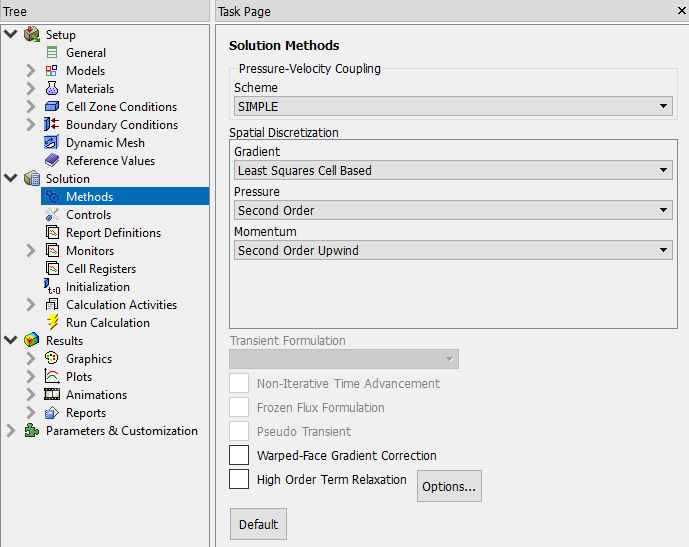
\includegraphics[width=0.4\textwidth,clip]{solution_methods.png}
\end{center}
\end{figure}

Select \bfr{Controls} in the \emph{Project Tree}. In the \emph{Task Page} you will now see a table with \bfr{Under-Relaxation factors}. Recall the \emph{Successive Over-Relaxation} method in Lecture Notes 4, where an over-relaxation factor ($\omega>1$) was introduced to accelerate the iteration process and reach faster convergence. Here \emph{Successive Under-Relaxation} is applied ($\omega<1$) which reaches convergence slower, but leads to a more stable solution. Finding the right relaxation factors is a largely empirical exercise and based on experience. The default values in Fluent are set to values that are near optimal for a large number of situations, we will therefore adopt the default values:
\begin{figure}[H]
\begin{center}
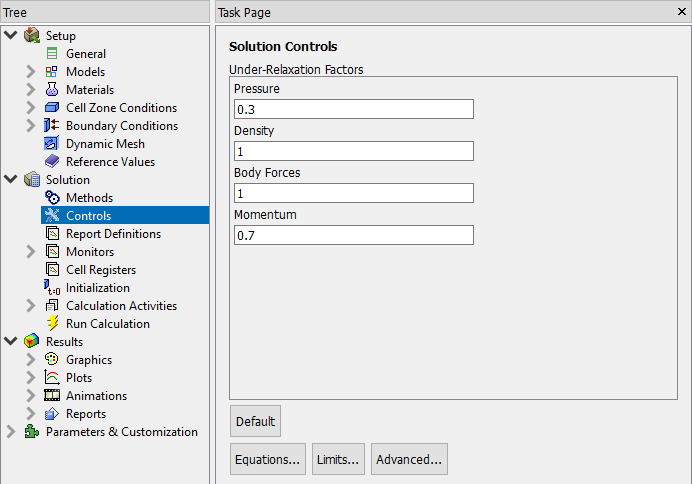
\includegraphics[width=0.4\textwidth,clip]{under_relaxation_factors.png}
\end{center}
\end{figure}

\subsubsection{Monitoring solution convergence}
\hl{add some comment here on residuals - can we refer to lecture notes?}

Double-click \bfr{Monitors} in the \emph{Project Tree} to show the various Monitor options and then double-click \bfr{Residual} which shows the Residual Monitor dialogue box. The monitors provide an overall view of the iteration convergence of the equations that we are solving (here continuity, x-velocity and y-velocity) at all nodes after every iteration. At every iteration the residual (Lecture Notes 4) is compared to the specified \bfr{absolute criteria}, if the residual is less then the specified criteria the solution of the equation is considered to be converged. In our case we are going to set all three convergence criteria (\bfr{Absolute criteria}) to 1e-6. Ensure that all other setting in the dialog box are set as follows:
\begin{figure}[H]
\begin{center}
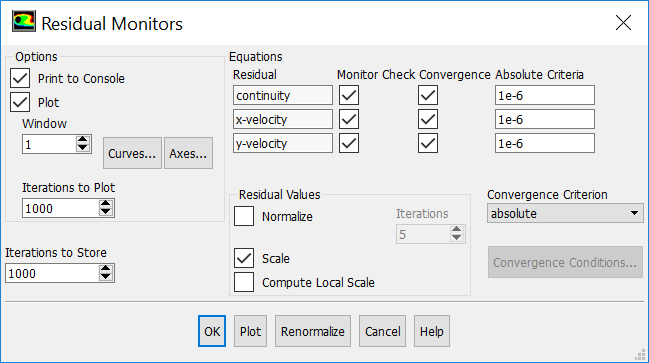
\includegraphics[width=0.6\textwidth,clip]{convergence_criteria.png}
\end{center}
\end{figure}

%Since we often are interested in a specific variable in our simulation, for example the force on a wall section of our model or the pressure at a specific location, it is very useful to monitor the convergence of this variable. It could for example be that the convergence of the variable of interest is already reached long before the residuals of the governing equations have reached their convergence criteria, and therefore the simulation could already be stopped in order to reducing the computational time. Here we will add a monitor for the drag coefficient on the pipe wall. Click \bfr{Create} in the \emph{task page} under \bfr{Residuals, Statistics and Force monitors} and select \bfr{Drag} from the drop down menu as shown below:
%\begin{figure}[H]
%\begin{center}
%\includegraphics[width=0.4\textwidth,clip]{drag_force_monitor.png}
%\end{center}
%\end{figure}
%Give the monitor a suitable name and select \bfr{pipewall} under wall zones, also tick the \bfr{Print to console} and \bfr{Plot} boxes under Options, then select \bfr{OK}.  Note that Fluent calculates the drag coefficient with respect to user-defined reference values for the density, velocity and area:
%\begin{equation}
%    C_\mathrm{D}=\frac{F_\mathrm{D}}{0.5\rho_\mathrm{ref} V_\mathrm{ref}^2 A_\mathrm{ref}}=\frac{\int\vec{\tau}_\mathrm{w}\vec{a}\mathrm{d}A}{0.5\rho_\mathrm{ref} V_\mathrm{ref}^2 A_\mathrm{ref}}
%\end{equation}
%The drag force $F_\mathrm{D}$ is calculated in Fluent by integrating the  wall shear stress $\vec{\tau}_\mathrm{w}$ over the wall area, here $\vec{a}$ indicates the direction in which the force is acting, which is in this case is the x-direction parallel to the pipe wall (note that we have set this \bfr{force vector} to (x,y)=(1,0) in the diagram above - in case of a vertical lift force this would have read (0,1) for example). Now go to \bfr{Reference Values} in the navigation pane and specify the reference Density and Velocity with the values given in the project description and set the Area equal to the wetted area of the pipe ($A_\mathrm{ref}=2\pi r L$).
%\begin{figure}[H]
%\begin{center}
%\includegraphics[width=0.3\textwidth,clip]{reference_values.png}
%\end{center}
%\end{figure}

\subsubsection{Initialisation}

Before we can run the simulation we first need to give all the variables at each node an initial value (our \emph{initial condition}, \hl{refer to lecture notes??}). In our case we only have three variable (pressure, axial and radial velocity) therefore we have three initial conditions to specify. As our initial condition we are going to specify a radial velocity of 1\,m/s in every cell in our flow domain. Double-click on \bfr{Initialisation} in the project tree, and select \bfr{Standard Initialization} in the \emph{Task Page}. Choose \bfr{inlet} in the \bfr{compute from} drop-down menu. Ensure that the values are defined as below and press \bfr{Initialize}.
\begin{figure}[H]
\begin{center}
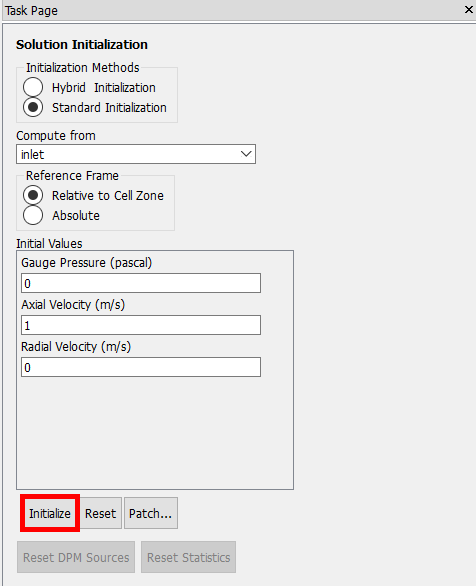
\includegraphics[width=0.4\textwidth,clip]{initialization.png}
\end{center}
\end{figure}


\subsubsection{Run the calculation}

Finally it is time to run our calculation! Before we do so however, we want to save a variable for later use in the post-processing stage which by default is not saved by Fluent. Go to \bfr{Files} in the \emph{menu bar}, select \bfr{Data File Quantities} and in the right column select \bfr{Skin Friction Coefficient} and click \bfr{OK}.
\\
Now select \bfr{Run Calculation} from the \emph{Project Tree}. We now need to set the \bfr{Number of Iterations}, which we set here to 100. Remember that we have also specified convergence criteria before, therefore our calculation will finish either when the specified number of iterations are completed, or when all the specified convergence criteria are met. Note that it is good practice to specify a small number of iterations initially (say 100) until you are sure that the solution will converge (this you can see from your residual monitors). This will avoid unnecessarily long computations in case of a non-converging iteration due to errors in the set-up. If you have verified that your simulation is converging after the initial iterations you can simply continue the simulation by pressing \bfr{Calculate} again (you can change the number of iterations if you want). While the calculation is running you can switch between the residual monitor and drag force monitor view in the top left corner of your \emph{Graphics Window}.
\\
\\
After about 76\,iterations the calculation stops since all the residuals have fallen below the specified convergence criteria of 1e-6. Note that although the console will display that the \emph{solution is converged} as shown below, this does not necessarily mean that the simulation is really converged! Remember that the solution criteria were defined by ourselves, so if we had put there some large numbers the simulation would probably have converged after a few iterations. We will therefore need to make the judgement ourself based on the residual history and the variable history. The converged simulation would include two factors: 1) a small residual and 2) negligible changes of our variable. Here we have set the drag coefficient as our monitor variable and we can see from the graphics window and in the console (fifth column) that our drag coefficient has reached a steady value after approximately 55\,iterations.
\\
\\
Now that the simulation is completed we can start with \emph{post-processing} of our results, or in other words displaying our results in figures, tables, animations etc. You can see in the \emph{Project Tree} that the Fluent Solver has an inbuilt post-processing features which you can find under \bfr{Results} in the \emph{Project Tree}. Although these features are fine to quickly display results some results while you are testing your set-up, the ease of use and functionalities are rather limited. We will therefore use the external pos-processer called \emph{CFD-Post}.
\\
Therefore, save your project and close the \emph{Fluent Solver}.

\begin{figure}[H]
\begin{center}
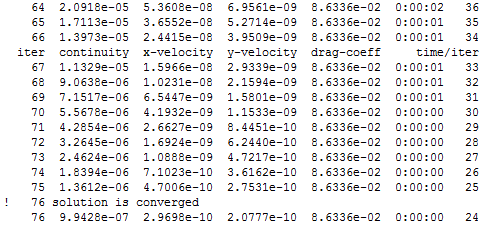
\includegraphics[width=0.4\textwidth,clip]{residuals_console.png}
\end{center}
\end{figure}

\subsection{Post-processing}\label{sec:postproc}

In this section we will display to make the the most common type of figures using \bfr{CFD-Post}, which are \emph{Vector Maps} (which show magnitude and direction of a variable in a 2D plane), \emph{Contour Maps} (which show magnitude of a variable in a 2D plane) and \emph{LinePlots} (which show the variable as a function of distance).

Drag the \bfr{Results} component in the \emph{Component Systems} to the \emph{Project schematic}, and connect the \bfr{Solution} cell from the Fluent component table to \bfr{Results} cell in the Results component table. Right-click on \bfr{Results} and select \bfr{update} from the drop-down menu.

\begin{figure}[H]
\begin{center}
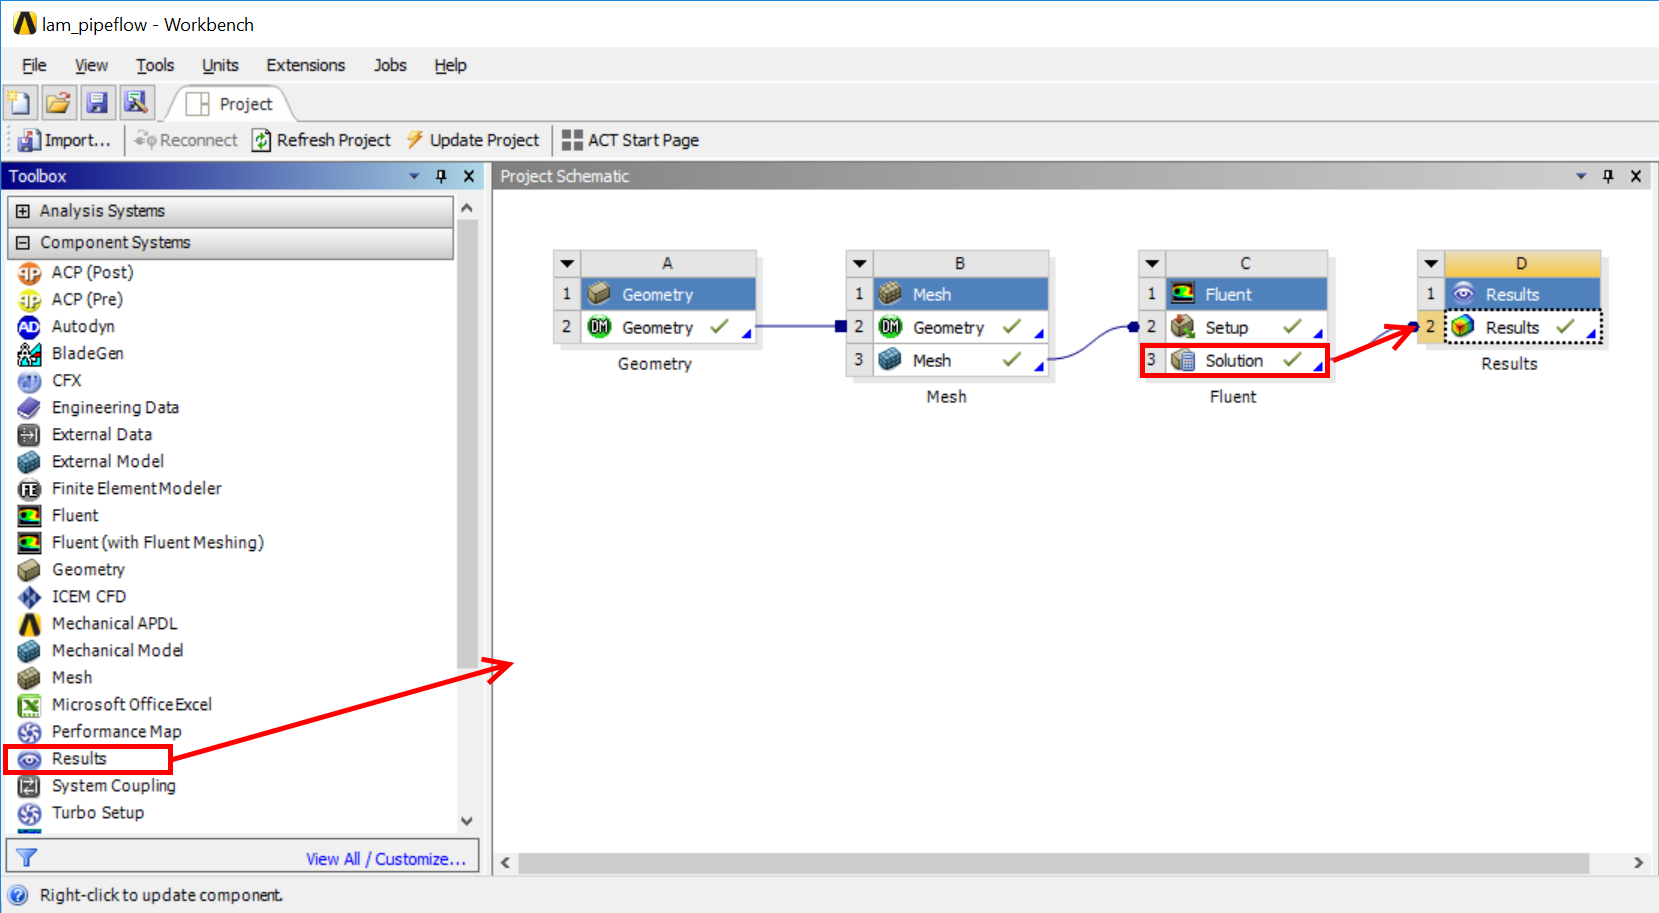
\includegraphics[width=0.45\textwidth,clip]{results_workbench.png}
\end{center}
\end{figure}

Double-click \bfr{Results} in the results component box, this will launch \emph{CFD-Post} which is the post-processing program which we will use to plot our results. The interface of \emph{CFD-Post} consists of the \emph{tree outline} and \emph{detailed viewer} on the left, the main window is called the \emph{viewer area}, here you can change the view in the different tabs on the bottom, and the \emph{toolbars} on top, of which the \emph{creation toolbar} contains the main functions for plotting results.

\begin{figure}[H]
\begin{center}
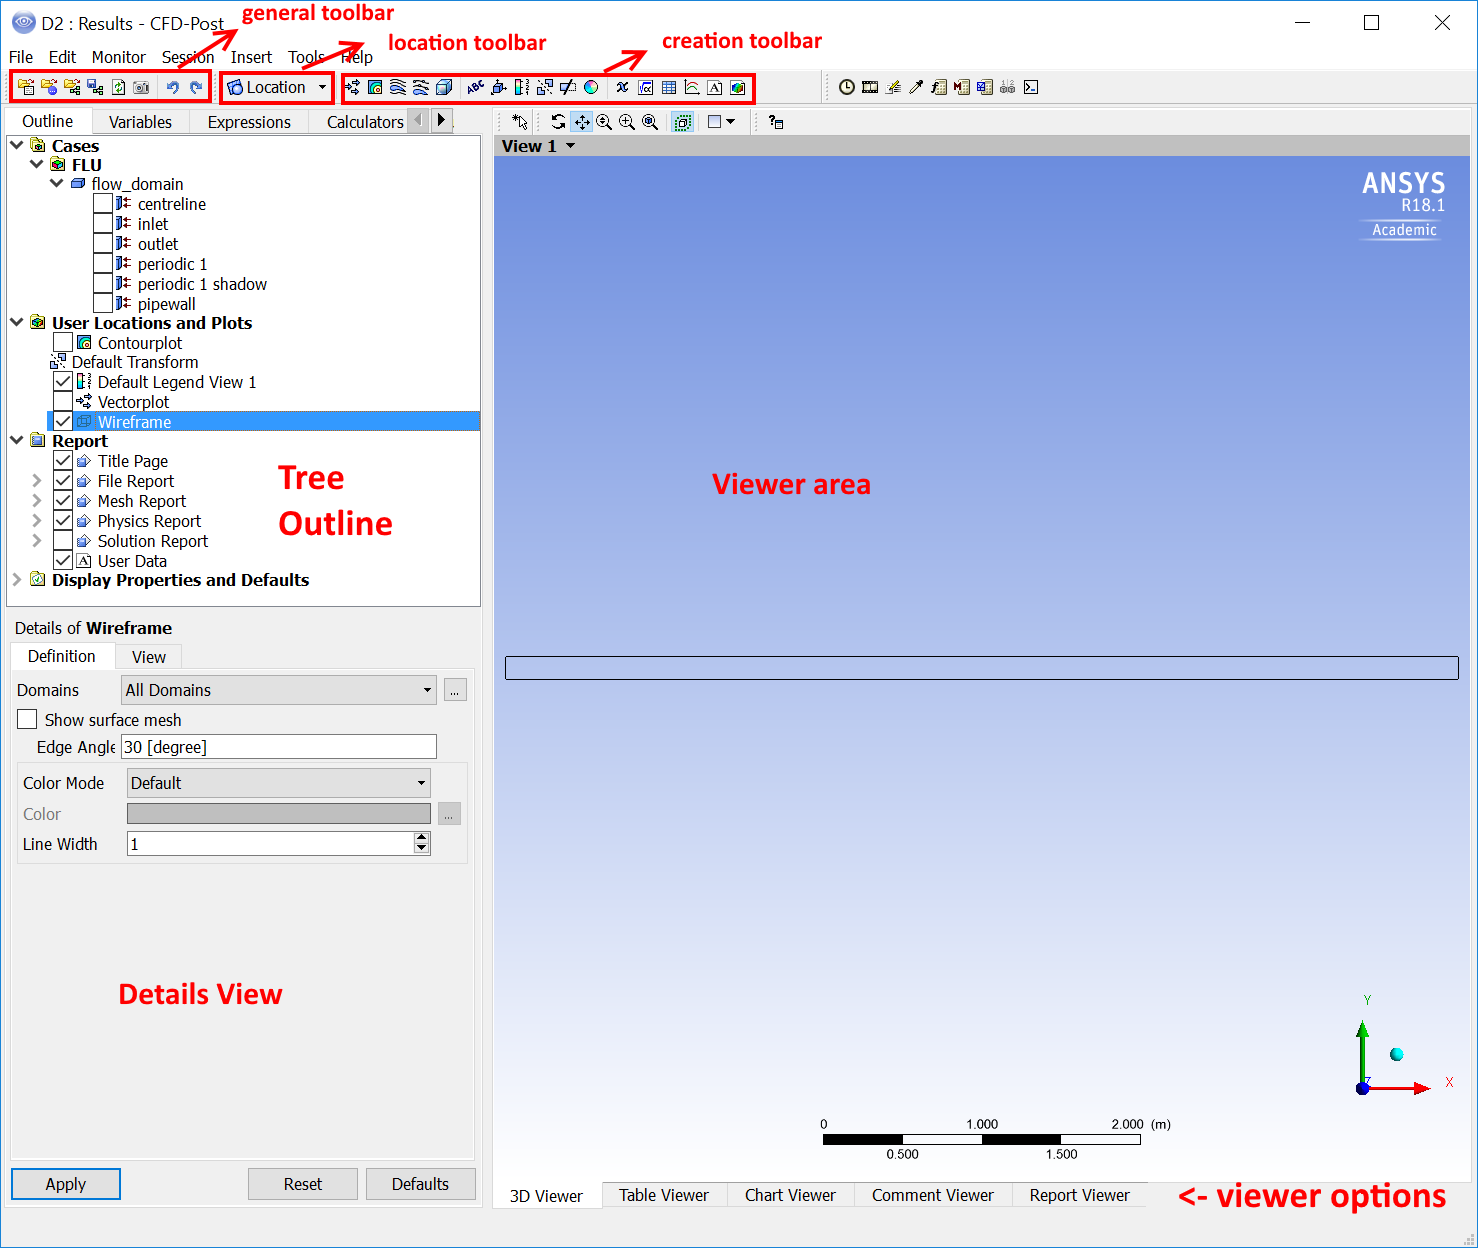
\includegraphics[width=0.7\textwidth,clip]{CFDPost_GUI.png}
\end{center}
\end{figure}

In the following subsection we will give step-by-step procedure to create \emph{velocity vectors}, a \emph{velocity magnitude contour}, \emph{velocity profiles} and to create a plot of the \emph{skin friction coefficient along the pipewall}.

\subsubsection{velocity vectors}

\begin{itemize}
\item click on the Z-axis to view the XY Plane
\item click on \bfr{periodic 1} under surface body in the \emph{tree outline}. Note that periodic 1 is the default name that CFD-Post gives to the interior of the flow
\item click the vector icon 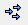
\includegraphics[width=0.4cm]{vector_icon.png} in the \emph{creation toolbar}, give a suitable name and click \bfr{OK}
\item select \bfr{periodic 1}  under location in the \emph{Details View}
\item in the \bfr{Symbols} tab change the symbol size to 0.2 (otherwise the vectors will appear too large) and click \bfr{Apply}
\end{itemize}

Note that only one half of the pipe cross-sectional area is displayed since we only did simulations for one half of our axisymmetric model. In order to display the bottom half as well double-click \bfr{Default Transform} in the \emph{Tree Outline},  untick \bfr{Instancing Info from Domain} in the \emph{Details View} and in the bottom (scroll-down) tick \bfr{apply reflection} and under Method select the \bfr{ZXPlane} and click \bfr{Apply}. Your vector plot  should now look like below (zoomed in on the inlet). To save a plot press the \includegraphics[width=0.4cm]{save_picture_icon.png} icon in the general toolbar, set the desired filename and format in the dialog box and press \bfr{Save}.

\begin{figure}[H]
\begin{center}
\includegraphics[width=0.5\textwidth,clip]{vector_plot.png}
\end{center}
\end{figure}

\subsubsection{velocity magnitude contours}\label{sec:velcontour}

\begin{enumerate}
\item click on the contour icon \includegraphics[width=0.4cm]{contour_icon.png} in the creation toolbar, give an appropriate name and click \bfr{OK}
\item in the \emph{Details View} select \bfr{periodic 1} under locations
\item change the the Variable from pressure to \bfr{velocity u} and click \bfr{Apply}
\item to increase the number of contours change \bfr{\# of Contours} to e.g. 50 and click \bfr{Apply} again
\end{enumerate}

The figure below show an example contour plot with 50 contours (zoomed in on the inlet). Note that for this figure the vector plot and WireFrame have been unticked under \bfr{User Locations and Plots} in the \emph{Tree Outline}. Note how the velocity is uniform at the pipe inlet (as set by our inlet boundary condition) but that it develops with x-distance showing a high velocity central region in the pipe and low velocity regions close to the pipewall. (Note that you can change the appearance of the legend in the details view of \emph{Default Legend View 1}.)
\begin{figure}[H]
\begin{center}
\includegraphics[width=0.5\textwidth,clip]{velocity_contour.png}
\end{center}
\end{figure}

\subsubsection{velocity profiles (velocity as a function of radial position)}
Here we are going to plot the velocity profile at the inlet and outlet of our pipe. To make these profiles we first need to specify the lines along which we want to plot our profiles.
\begin{enumerate}
\item create a line by clicking \includegraphics[width=1.7cm]{Location_icon.png} in the \emph{creation toolbar} and select \bfr{Line} and name it \bfr{Pipe Inlet}
\item in the \emph{Details View} you can enter the (x,y,z) coordinates for the two points that make up the line, enter (0,0,0) for point 1 and (0,0.15,0) for point 2 and press \bfr{Apply}. Set the number of samples to 8, i.e. equal to your mesh size along the inlet and outlet. Note that increasing the amount of samples beyond the mesh size does not lead to more detail in your plots since the results are simply linearly interpolated between the calculation points.
\item repeat the steps above to create the \emph{pipe outlet}, with coordinates (6,0,0) for point 1 and (6,0.15,0) for point 2.
\item check the location of both lines in your view area, you might need to untick the previously generated velocity vectors and contour in the project tree to be able to see them properly.
\item select the chart icon \includegraphics[width=0.4cm]{chart_icon.png} from the \emph{creation toolbar}, name it velocity profiles and select \bfr{OK}.
\item go to to the \bfr{data series} tab in the \emph{Details View} and under location select \bfr{pipe inlet}, also under name type pipe inlet.
\item select the \bfr{X-axis} tab and select \bfr{Velocity u} as variable
\item select the \bfr{Y-axis} tab and select \bfr{Y} as variable and select \bfr{Apply}
%\item go back to the \bfr{Data Series} tab and press the \includegraphics[width=0.4cm]{new_icon.png} symbol which adds a new data series to the existing plot, now repeat the steps above to plot the velocity profile along the pipe outlet.
\end{enumerate}
Your velocity profile plot should look as below.
\begin{figure}[H]
\begin{center}
\includegraphics[width=0.6\textwidth,clip]{velocity_profiles.png}
\end{center}
\end{figure}

The data can be exported to a comma-separated-file (\texttt{*.csv}), which can be imported in Excel or Matlab\footnote{using the \texttt{csvread} command} to compare your simulated data to other types of data (e.g. analytical or experimental data). In order to export the data press \bfr{Export} in the Details View of your velocity profiles that have just been created (note that the velocity profiles are listed under  \bfr{Report} in the project tree.

\subsubsection{skin friction coefficient along the pipe wall}

Here we will plot the skin friction coefficient (=normalised wall shear stress) along the pipe wall. The skin friction coefficient in Fluent is (similar to the drag coefficient) calculated with respect to the user-defined reference values for the density and velocity as follows:
\begin{equation}
    c_\mathrm{f}=\frac{\tau_\mathrm{w}}{0.5\rho_\mathrm{ref}U^2_\mathrm{ref}}
\end{equation}

We had already set the correct reference values in order to monitor our drag force coefficient and we have already told Fluent to export the skin friction coefficient so we can now plot the skin friction coefficient along the pipe wall as follows:
\begin{enumerate}
\item create a line called ``pipe wall'' starting at (0,0.15) and ending at (6,0.15)
\item select the chart icon from the create toolbar, name it ``skin friction coefficient'' and press \bfr{OK}
\item in the \emph{Details View} select pipe wall under location in the \bfr{Data series} tab
\item in the \bfr{X-axis} tab select \bfr{X} as the variable and under \bfr{Y-axis} select \bfr{skin friction coefficient} and click \bfr{Apply}
\end{enumerate}

\begin{figure}[H]
\begin{center}
\includegraphics[width=0.6\textwidth,clip]{skin_friction_coefficient.png}
\end{center}
\end{figure}


\subsection{Verification \& Validation}

Although we have now produced very nice colorful results it is essential to perform a \emph{verification} and \emph{validation} checks to get more confidence in our results. The verification checks essentially demonstrate whether we have solved our equations correctly, ie whether the numerical procedures are done correctly. However, verification  only tells us that we have numerically solved the equations correctly, we could of course still have the wrong set of equations to describe our physical model! Therefore still need to \emph{validate} our model, which can be done by comparing it to analytical or experimental results. Most CFD cases involve complex flow conditions for which analytical results do not exist hence validation is generally performed using experimental data. For our flow problem, laminar flow in a pipe, an exact analytical solution exists so we are going to compare against the analytical solution.


\subsection{Verification}

\begin{itemize}
\item The first (and often overlooked) step involves ``common sense'' checks, or in other words did we get what we more or less expected to happen. So in this case is the flow from left to right (ans:yes)? Does the velocity profile at the outlet resemble our expectations, i.e. a parabolic shaped profile with larger velocities in the centre of the pipe and smaller towards the wall (ans:yes)? We also need to check whether our boundary conditions are satisfied in our results. In our case the inlet boundary condition was a uniform velocity of 1\,m/s and no-slip (u=0\,m/s) along the pipewall. We can verify in our results that these boundary conditions satisfied, for example in the velocity contour we made in section~\ref{sec:velcontour}.
\item Is the conservation of the governing equation satisfied? Or in other words, did we conserve mass (continuity eq), momentum (in x- and y-direction), energy (if we had used the energy equation in a heat transfer problem), etc. In this case we are only going to check whether mass is conserved, since conservation of momentum is a bit more elaborate. Close \emph{CFD-Post} in case you still had it open, then re-open the \bfr{Fluent Solver} and run the simulation again. Now in the \emph{Project Tree} go to \bfr{Results$\rightarrow$Reports} and then double-click on \bfr{Fluxes}. Then select the four boundaries of our model ``domain'' and click \bfr{Compute} as follows:
    \begin{figure}[H]
    \begin{center}
    \includegraphics[width=0.6\textwidth,clip]{mass_cons.png}
    \end{center}
    \end{figure}

    The results window now shows the mass fluxes going across each boundary, with positive values meaning that mass is entering our domain and negative that it is leaving our domain. As expected mass is only entering the inlet and leaving the outlet, there is no mass flux across the pipewall or the centreline. The difference between the mass going in and out of domain is given at the bottom and it shown that this a very small number of $O(10^{-11})$ compared to the flux entering the control volume $O(10^{-2})$. We can therefore conclude that mass is conserved, which gives more confidence that we solved our equations accurately.
\item \hl{check linearization error due to number of iterations}
    \begin{figure}[H]
    \begin{center}
    \includegraphics[width=0.6\textwidth,clip]{residual_sensitivity.png}
    \end{center}
    \end{figure}

\item Now we establish that our chosen mesh size is small enough that spatial discretization error has reduced sufficiently such that it does not significantly alter our results. Or in other words, increasing the amount of cells in our domain should not alter our results anymore. We can then say that our solution has become \emph{mesh-independent}.Make a new mesh with double the amount of divisions in the radial direction (16 instead of 8). In order to do this simply make a copy of your mesh in the workbench (right-click the original mesh and select \bfr{duplicate}), then drag the original geometry to your new mesh, and open the \emph{Meshing} program to adjust the number of radial divisions and then click \bfr{Update} to update your new mesh. Then duplicate the Fluent solver in your workbench and connect this to your new mesh, run the fluent solver again and make sure that the residuals are converged (it will take about 128 iterations, so you need to increase the number of iterations). Then connect the duplicated solution to your previous results component (this will show both solutions in the plots you previously made). Your workbench should look like (note it is good practice to give the components a sensible name):

    \begin{figure}[H]
    \begin{center}
    \includegraphics[width=0.6\textwidth,clip]{workbench_finemesh.png}
    \end{center}
    \end{figure}

    Repeat the exercise for a mesh of 24 division in radial direction and compare velocity profiles at the outlet in \emph{CFD-Post}:
    \begin{figure}[H]
    \begin{center}
    \includegraphics[width=0.6\textwidth,clip]{Mesh_sensitivity.png}
    \end{center}
    \end{figure}
    It is shown that increasing the mesh from 600\,cells to 1200\,cells has changed the results slightly, in particular the maximum velocity along the centreline has increased. Further increasing the mesh to 1800\,cells did not alter the results significantly (green and blue line practically overlap), hence the results have become independent of the mesh size (the spatial discretization error has become so small that we do not notice it). For the remaining calculations we can therefore use the mesh size of 1200\,cells. Note that in this case we have checked the mesh sensitivity only for the velocity profile at the outlet, which in our case the main result of interest. Of course, if some other quantity is the variable of primary interest (e.g. the drag force), then typically you would determine the mesh sensitivity based on this variable. For many CFD applications in practice, which may consist of millions of cells, the final mesh choice is often a balanced decision between which error can be accepted and the extra computational time (=cost!) associated with a more accurate mesh.
\end{itemize}


%%%
%%% ASSIGNMENT 1: Validation
%%%
\section{ASSIGNMENTS}% 1: Validation Procedure for Section~\ref{Section:LaminarPipeSimple}}
\subsection{Assignment 1: Validation Procedure for Section~\ref{Section:LaminarPipeSimple}}
%\subsection{Validation (Exercises)}

\begin{enumerate}
   \item Compare the results (Section~\ref{Section:LaminarPipeSimple}) obtained from both, original and new mesh (\hl{Section XX}), with the theoretical velocity profile for fully-developed laminar pipe flow:
      \begin{equation}
          u(r)=2U\left(1-\frac{r^2}{R^2}\right),
      \end{equation}
where $r$ is the radial coordinate, $U$ is the average velocity across the pipe cross-sectional area and $R$ is the pipe radius. 
       \begin{enumerate}
          \item You can download experimental data from \textattachfile{u_prof_analytical.txt}{\underline{here}} and save it to your \emph{Homedrive};
          \item The first column in this file is the velocity in m/s and the second column the radial coordinate in m; 
          \item You can add this data to your plot of the velocity profile in \emph{CFD-Post} as follows: 
            \begin{enumerate}
                 \item From the \emph{Project Tree}, double-click the graph where you previously made your velocity profile;
                 \item From the \emph{Details View}, select the \emph{Data Series} tab and click \includegraphics[width=0.5cm,clip]{new_symbol.png} to a add a new data series;
                 \item From the \emph{Data Source}, select \bfr{File} and then browse for the \texttt{*.txt} file which you just saved to your \emph{homedrive} (in the import dialogue box you may need to change to file type to \emph{text files});
                 \item Then click \bfr{Apply} to load the data. You can change the name of the data-series to something sensible, e.g. \emph{analytical}. 
            \end{enumerate}
      \end{enumerate}
Is the numerical simulation validated?

   \item Plot the pressure along the axis centreline. Use the following relationship between pressure loss and average velocity to obtain the skin friction coefficient: 
\begin{equation}
    \Delta P=c_\mathrm{f}\frac{2L\rho U^2}{D}
\end{equation}
Calculate the skin friction coefficient for the entire pipe length ($x=0-6$\,m). Compare the results with the skin friction coefficient for fully developed laminar pipe flow:
\begin{equation}
    c_\mathrm{f}=\frac{16}{\Rey}
\end{equation}
   \item The \emph{entrance region} of the pipe is the region after the inlet where the boundary layer on the side wall is still growing. Once the boundary layer has reached the pipe centreline the velocity profile does not change with x-position anymore, i.e  $\partial u/\partial x=0$. The length of the entrance region, $L_\mathrm{e}$, is often taken as $L_\mathrm{e}\approx0.06D\Rey$. Calculate the skin friction based on the pressure drop in the region ($x=L_\mathrm{e}-6$\,m), compare your results to the theoretical value for fully developed flow.
\end{enumerate}


%%%
%%% ASSIGNMENT 1: Validation
%%%
\subsection{Assignment 2: Start-up Couette Flow}

In this section, we are going to simulate the start-up of a flow between two parallel plates which you have previously considered in Tutorial\,3 and Practical\,1a. Initially both plates and the fluid between them are at rest. At time equal zero ($t=0$), the upper plate starts moving with a constant velocity, $u_0$, as indicated below. Previously, we considered this as 1D problem by modeling one vertical profile of length $L$. Numerical simulations in Fluent need to be either 2D or 3D, therefore we are considering it as a ``box'' of fluid with dimension $L\times 2L$.

\begin{figure}[H]
\begin{center}
\includegraphics[width=0.7\textwidth,clip]{start_up_flow.png}
\end{center}
\end{figure}

Setting up this problem in Fluent is very similar to the laminar pipeflow problem, with the exception:
\begin{enumerate}
   \item  we are now dealing with a planar model domain (instead of axisymmetric), it is a \emph{transient} simulation (because $\frac{\partial\left(\cdot\right)}{\partial t}\neq0$ in the governing equations), and;
   \item the inlet and outlet boundary conditions are \emph{periodic} (because we essentially simulate a small element of an infinitely long domain);
   \item Thus, the main differences are:

\begin{enumerate}
\item Create the geometry and the mesh for this problem with dimensions as specified in practical\,1a. Choose $\Delta x =1$\,mm, i.e. one cell in $x$-direction. Don't forget to name your boundaries in the Meshing.
\item Solver: In the \emph{General} settings in Fluent set the Solver to \emph{Planar} and \emph{Transient}.
\item Fluid: Create a fluid with the specifications that satisfy the required kinematic viscosity.
\item Boundary conditions: set the top and bottom wall boundary conditions as specified in the assignment. 
    \begin{itemize}
       \item Click anywhere in the console and hit the enter key on your keyboard, know \texttt{>} should have appeared in the console. Type the following in the console 
       \begin{center}
            \texttt{grid/modify-zones/make-periodic}
       \end{center}
 and hit enter. The next line in the console will say  
       \begin{center}
            \texttt{Periodic zone [()]},
       \end{center}
which is asking you to indicate the Periodic zone.
       \item In our case, we want our Inlet to be the period zone, you can now type the name of your inlet (which may be \emph{inlet}), or you can use the ID, you can find the ID in the \emph{boundary conditions} task page:
 \begin{figure}[H]
\begin{center}
\includegraphics[width=0.4\textwidth,clip]{BC_ID.png}
\end{center}
\end{figure}
  So in this case I can type either \emph{inlet} (name) or \emph{5} (ID) and then hit enter.
       \item The next line will ask for the \emph{shadow zone}, which is the outlet of our domain in this case, so type the appropriate name or ID.
       \item In the subsequent lines type \texttt{no}, \texttt{yes} and \texttt{yes}. The console will now indicate that one zone has been deleted and that periodic zones are created.
       \item In the boundary conditions \emph{Task Page} you can now see that the inlet boundary condition \emph{type} has changed to \emph{Periodic} and that the outlet boundary condition has disappeared. In the bottom of the boundary conditions \emph{Task Page} you can now see that you can click the \emph{Periodic conditions ...} to set the period boundary condition (which was not selected previously, see figure above).
       \item Here we set the periodic boundary condition to specified pressure gradient of 0\,Pa/m (note that we actually have a zero-pressure gradient flow in this case, because the moving top plate is driving the flow, not the pressure!).
    \end{itemize} 
    
\item under \emph{Solution$\rightarrow$Methods} tick the \emph{Non-Iterative Time Advancement} box. Leave the \emph{Monitors} at their default values.
\item Initialise your results, and set the Time Step Size to the same timestep used in your Matlab simulation. 
\end{enumerate}

    \item Task: The start-up flow problem is a classic fluid mechanics problem that can be derived from the Navier-Stokes equations and is defined as
       \begin{displaymath}
           \frac{\partial u}{\partial t} = \nu \frac{\partial^{2}u}{\partial y^{2}},
       \end{displaymath}
       where $\nu$ is the kinetic viscosity, subjected to the following initial and boundary conditions,
       \begin{displaymath}
           \begin{cases}
               u(y,0) = 0, \;\;\;\;&  0 < y < L; 
           \end{cases}
       \end{displaymath}
       

can be derived from the 
\begin{enumerate}
   \item From the Navier-Stokes equations
   \item Run numerical simulations for 0.01\,s, 0.1\,s and 1\,s, and plot $u_{x}/u_{0} \times y/L$;
   \item Compare $u_\mathrm{x}$ from these simulations to Matlab results obtained in Practical\,1a. 
\end{enumerate}
Note that once you have made a graph in \emph{CFD-Post} you can export the data (by clicking \includegraphics[width=1.1cm,clip]{export_icon.png} in the \emph{Details View}) to a comma separated value file (\texttt{*.csv}) or a text file (\texttt{*.txt} or \texttt{*.dat}) which you can read into matlab (see \texttt{csvread} or \texttt{dlmread} commands). Alternatively, you can add the Matlab data to a text file and load it into \emph{CFD-Post} following the procedure described in the pipe flow case;
\end{enumerate}


\subsection{Exercises}

\begin{enumerate}
\item Run numerical simulations for 0.01\,s, 0.1\,s and 1\,s and compare $u_\mathrm{x}$ to your Matlab results obtained in practical\,1a. Note that once you have made a graph in \emph{CFD-Post} you can export the data (by clicking \includegraphics[width=1.1cm,clip]{export_icon.png} in the \emph{Details View}) to a comma separated value file (\texttt{*.csv}) or a text file (\texttt{*.txt} or \texttt{*.dat}) which you can read into matlab (see \texttt{csvread} or \texttt{dlmread} commands). Alternatively, you can add the Matlab data to a text file and load it into \emph{CFD-Post} following the procedure described in the pipe flow case. 
\item 

\hl{any more exercises that we can do? verification exercises? increase mesh and compare? check for mass continuity (=no need because of periodic BC's)}
\end{enumerate}



\vspace{2cm}
Submit (via MyAberdeen)\\
For practical 1a (29 Sept) and 1b a \emph{single} document (MsWord document or pdf-file) with the graphs requested, a discussion of the various issues, and answers to all the questions posed. Graphs directly obtained from Fluent need to be exported by clicking the \includegraphics[width=.4cm]{export_fig_icon.png} button, do not make direct screen copies of your graphs. Other graphs can be made in Excel, Matlab etc.
\\
\\
Deadline: 11$^\mathrm{th}$ October 23:59hrs

\end{document} 
